%-----------------------------------------------------------------------------%
% Format and styling in this file originally created by 
% Carl E. Svensson 2010, updated by Adam J. Carmichael 2011
%-----------------------------------------------------------------------------%
%
%- Document Makeup -----------------------------------------------------------%
%- (01) Notes from template author
%- (02) Document Class and Options
%- (03) Standard package includes and options
%- (04) Custom Definitions and Alterations
%- (05) Custom Commands
%- (06) Document title and other metadata
%- (07) Start Document Content
%- (07a) Misc Config
%
%
%- (01) Notes from carneeki@ -------------------------------------------------%
% NEATNESS:
%  Please keep the TeX neat. Best ways to do this:
%  (01) Don't indent
%  (02) Keep inside of 80 characters (it makes for nicer editing on small
%       laptops).
%  (03) Avoid whitespace between \section{} and other document elements. We
%       have %%%% comments for a reason!
%  (04) Use 2 (that's TWO) space characters to indent. NEVER use tab unless
%       your editor converts to to space chars.
%  (05) Maintain customisations in their respective sections.
%  (06) Comment everything. Bandwidth and diskspace are cheap these days, and
%       TeX compresses pretty nice. Anything else is the BAD kind of laziness
%       on your part.
%
% MULTILINE EQUATIONS:
%  Use \begin{align} instead of \begin{eqnarray}...
%  Details as to why are found at (tl;dr : it's just better...):
%  http://texblog.net/latex-archive/maths/eqnarray-align-environment/
% 
% BIBLIOGRAPHY: 
%  -> URLS: to generate the GUID for a reference that is for a URL, paste
%     the URL into goo.gl and then take only the suffix portion.
%
%  -> Wikipedia citations, simply copy + paste the citation from the
%     menu on the LHS.
%
%
%- (02) Document Class and Options -------------------------------------------%
\documentclass[
%  pagesize,
  a4paper,
  pdftex,
%  fontsize=11pt,
%  draft=true,
  twoside,
]{book}
%
%
%- (03) Standard package includes and options --------------------------------%
\usepackage[Lenny]{fncychap}
%\usepackage[Bjornstrup]{fncychap}
%\usepackage{draftwatermark} % draft watermark. Comment these 2 lines in final
%\SetWatermarkLightness{0.9} %
\usepackage{amsmath}       % amsmath & amssymb are almost ALWAYS required.
\usepackage{amssymb}       %
\usepackage{gensymb}       % for the degrees circle!
%
%\usepackage{verbatim}     % multiline commenting ( c++ equiv /* ... */ )
%
\usepackage{color}
\usepackage{xcolor}         % pdflatex
\definecolor{neekiRed}{RGB}{172,40,41}
\definecolor{neekiBlue}{RGB}{62,70,157}
\definecolor{neekiGreen}{RGB}{39,171,39}
\definecolor{neekiPurple}{RGB}{105,39,171}
%
\usepackage{geometry}      % option for altering page dimensions if needed
%\usepackage[pdftex]{graphicx} % including image files for figures (ie
                              % non-[E]PS)
%                          % valid types: jpeg, png, pdf
\usepackage{wrapfig}       % the figures themselves
\usepackage[numbers,
square,
longnamesfirst
]{natbib}                  % prettybib
\usepackage[pdftex]{hyperref} % clickable TOC and refs
%\usepackage[all]{xy}      % category theory helpers
%\xyoption{all}            % category theory helpers
%\input xy                 % category theory helpers
\usepackage{tikz}        % easy graphic thing
\usepackage{tabularx}    % easy tables
\usepackage{url}         % easy urls
\usepackage{multirow}    %
\usepackage{lipsum}      % autogen placeholder text
%
%- (04) Custom Definitions and Alterations -----------------------------------%
\usepackage[T1]{fontenc} % font-doohickey
%\usepackage{tgadventor}  % font
%\usepackage[math]{iwona} % font
\usepackage{kurier} % font

%
\linespread{1.5} % carneeki@ use approx 150% line spacing just like MaxDesign.
\hypersetup{
  % DO NOT CHANGE THESE
%   pdftitle={\metaTitle},
%   pdfauthor={\metaAuthorShort},
%   pdfsubject={\metaSubject},
%   pdfkeywords={\metaKeywords},
  pdfcreator={LaTeX},
  pdfproducer={LaTeX},
  pdftoolbar=false,
  % But change these to taste:
  pdffitwindow=false,   % window fit to page when opened
  pdfstartview={Fit},   % fits the width of the page to the window
                        % all (useful) opts: Fit, FitH, FitV,
  pdfpagelayout=TwoPageLeft,
  pdfnewwindow=true,    % open links in new window
  colorlinks=true,      % false = boxed links; true = colored links
  linkcolor=neekiRed, % color of internal links
  citecolor=neekiBlue, % color of links to bibliography
  filecolor=red, % color of file links
  urlcolor=red  % color of external links
}
%
%- (05) Custom Commands ------------------------------------------------------%
% MATH
\newcommand{\derivative}[1][x]{\frac{\mathrm{d}}{\mathrm{d}#1}}
\newcommand{\deriv}[2]{\frac{\mathrm{d}#1}{\mathrm{d}#2}}
\newcommand{\ndeg}{^\circ} % the degrees symbol
\newcommand{\neqref}[1]{\text{(#1)}}
% trig
\newcommand{\isin}{\sin^{-1}}
\newcommand{\icos}{\cos^{-1}}
\newcommand{\itan}{\tan^{-1}}
% DMTH
\newcommand{\lxor}{\oplus}
\newcommand{\lxnor}{\lnot\lxor}
\newcommand{\true}{(\mathbb{T})}
\newcommand{\false}{(\mathbb{F})}
% GENERAL
\newcommand{\qedbitches}{\qed}
\renewcommand{\labelenumi}{(\alph{enumi})}
\renewcommand{\labelenumii}{(\roman{enumii})}
%
%- (06) Document Title and other metadata ------------------------------------%
%
\title{
  The MATH130 Student's Guide to Chen and Duong's MATH130 notes.
}
%
\author{
  Adam J. Carmichael \\
  Undergraduate Student \\
  Department of Electronic   Engineering\\
  Macquarie University\\
  Sydney, Australia 2109\\
  Email: \url(adam.carmichael@ieee.org) \\
\and
  Carl E. Svensson \\
  PhD Candidate \\
  Department of Electronic   Engineering\\
  Macquarie University\\
  Sydney, Australia 2109\\
  Email: \url(carl.svensson@ieee.org) \\
} % author END Brace
%
%- (07) Start Document Content -----------------------------------------------%
\begin{document}
%- (07a) Misc Config ---------------------------------------------------------%
%
\maketitle
%
%\begin{abstract}
%This document is a guide written primarily by a MATH130 student and his friend
%in the 2 week study period between end of class and the examination of
%semester 1, 2011. It is an interpretation that aims to make the very thorough
%notes of Chen and Duong easier and more accessible to the rest of us.
%\end{abstract}
%-----------------------------------------------------------------------------%
%- Acknowledgments -----------------------------------------------------------%
%-----------------------------------------------------------------------------%
\chapter{Copyright and Terms of Use, and Other Bits}
\label{chap:Copyright}
\section{Copyright}
This work has been authored mostly by Adam Carmichael,
\url{adam.carmichael@students.mq.edu.au} and is mostly his copyright material,
except where noted.

Use of the source of this work is licensed under a Creative Commons
Attribution NonCommercial NoDerivs 3.0 Unported License. The full details of
this license are available from
\url{http://creativecommons.org/licenses/by-nc-nd/3.0/}.

I chose a NoDerivs suffix as it is trivial to take this work, and push
``compile'' button in any \LaTeX~editor and generate a textbook to take to a
publisher. It would be unfair (on myself, as well as everyone who helped) to
allow that to happen. Should you wish to generate a textbook, please contact the
author to discuss textbook licensing.

If you wish to make ammendments to details, by all means, fork the code, and
send me a patch containing your changes, or a ``pull request'' (or both). You
will get a mention in the acknowledgements, and if a publisher wants a textbook
you will also get a reward commensurate with the changes you provide.

\section{Terms and conditions of use}
This work is an open source project. It strives to be technically correct and
accurate, though, it may not be.

\section{A cautionary word}
I've failed MATH130 at least twice. I've been pissed with the Maths
department. I've written most of this book whilst ropable at them for not doing
it themselves. This may not be the best resource, but they haven't really done a
good enough job of organizing their resources, so resources are limited. Please
attend lectures, tutorials and practicals. Go ask your teachers, tutors,
professors, lecturers, and friends questions and be active in classes. It is
said the only way to learn math is to do math. If you say ``screw math'', it
\emph{will} screw you\footnote{And it might screw you anyway\ldots}.

\section{Typesetting}
This book has been typeset in \LaTeX~using a Lenovo X201 Tablet running
Microsoft Windows 7, Eclipse Indigo, TeXlipse and MikTex 2.9 64-bit beta. I've
been drinking copious amounts of energy drinks and coffee; if you would like to
become a sponsor and have your name mentioned here, let me know.

The source is presently available from
\url{https://github.com/carneeki/Grokking-MATH130}. You should be able to find
updates of the PDF at \url{http://goo.gl/X14C4}. The PDF may not always match
the latest source, but you can always compiled the PDF yourself.

Additionally, most URLs in the PDF should be clickable. URLs in footnotes may
not be; this is something that needs to be debugged.

\section{Introduction}
\label{sec:Introduction}
%A long long time ago, in an office far far away, a bright mathematician decided
%to come up with a method for making sure MATH students at Macquarie had no
%social life by ensuring our mathematics was up to scratch. Unfortunately, some
%of us decided to turn mathematics into a social affair by interpreting that
%bloke's notes in an easy manner.
In 1999 a pair of elite mathematicians\footnote{Chen and Duong} decided to
write some notes for a subject they knew plenty about. The notes proved
difficult to understand by some and could have been made easier by means of an
introduction in plain simple English. Today they survive as reference documents
on Rutherglen. If you can find them, and you read them, and you have this
guide, then maybe you can pass MATH130.\\
\emph{(To be read whilst playing the introduction to the A-Team).}\\
\\
Typically the syllabus is broken into two streams, calculus and algebra. This
gives rise to certain problems if algebra falls behind calculus because
there are prerequisites in algebra to solving some calculus problems. As such,
these notes will be arranged such that the algebra material is covered first.

\tableofcontents
%-----------------------------------------------------------------------------%
%- Algebra :: Types of Numbers & Symbols Used --------------------------------%
%-----------------------------------------------------------------------------%
\chapter{Types of Numbers \& Symbols Used}
\label{chap:TypesOfNumbersAndSymbolsUsed}
Maths is pretty much a written language used to convey what people want to do
to numbers, variables, or other bits of information. There are various types
of numbers, and sometimes special symbols are used to denote what conditions
must be placed on those numbers.
\section{Types of Numbers}
\label{sec:TypesOfNumbersUsed}
Table \ref{tab:TypesOfNumbers} outlines the types of numbers encountered in
MATH130, followed by a few additional types of numbers that are handy to bear
in mind.
\begin{table}[!htb]
\label{tab:TypesOfNumbers}
\begin{tabularx}{\linewidth}{| c | l | c | X |} \hline
  Symbol & Name & In MATH130 & Description \& Example \\ \hline \hline
  $\mathbb{N}$ & Natural Number     & Yes & Any whole number greater than
                                            zero. $1, 2, 3 $ \\ \hline
  $\mathbb{R}$ & Real Numbers       & Yes & Any number along a continuum.
                                            $-1, 0, 1, \pi $ \\ \hline
  $\mathbb{Z}$ & Integers           & Yes & Any whole number.
                                            $-1, 0, 1 $ \\ \hline
  $\mathbb{I}$ & Irrational Numbers & Yes & Numbers which cannot be expressed
                                            as a fraction.
                                            $e, \pi, \sqrt[2]{2} $ \\ \hline
  $\mathbb{Q}$ & Rational Numbers   & Yes & Numbers which can be represented as a
                                            fraction.
                                            $ \frac{1}{2}, 1, \frac{0}{4} $
                                            \\ \hline
  $\mathbb{C}$ & Complex Numbers    & Yes \footnote{Only a brief introduction
  to complex numbers is covered, and traditionally it is at the end of MATH130
  incase there isn't enough time to cover it.}
                                            & Numbers which have both a real
                                            part, and an imaginary part.
                                            $ \frac{2}{-1} = i $ \\ \hline
  $\mathbb{P}$ & Prime Numbers      & No \footnote{They come up, but really, it's
 only in factorization.}
                                            & Numbers which are divisible only
                                            by themselves and one.
                                            $1, 2, 3, 5, 7, 11, 13 $ \\  \hline
\end{tabularx}
\caption{Types Of Numbers}
\end{table}

\section{Types of Symbols}
\label{sec:TypesOfSymbols}
Table \ref{tab:TypesOfSymbols} outlines the types of symbols you are likely
to encounter in MATH130. This list is partially built from \citet{IjPb7}.
\begin{table}[!htb]
\label{tab:TypesOfSymbols}
\begin{tabularx}{\linewidth}{| c || c | X |}
  \hline
  Symbol & Example & Read as \\ \hline \hline
  $ \in    $ & $ x \in    \mathbb{R} $ & x is an element of $\mathbb{R}$ (real
                                       numbers)                       \\ \hline
  $ \notin $ & $ x \notin \mathbb{R} $ & x is not an element of $\mathbb{R}$
                                       (real numbers)                 \\ \hline
  $ \cup   $ & $ \mathbb{I} \cup \mathbb{Q} \in \mathbb{R}$
                                       & The set $\mathbb{I}$ (irrational
                                       numbers) and $ \mathbb{Q} $ (rational
                                       numbers) are in set $\mathbb{R}$ (real
                                       numbers).                      \\ \hline
  $ =       $ & $ x = y       $ & x is equal to y                     \\ \hline
  $ \neq    $ & $ x \neq    y $ & x is not equal to y                 \\ \hline
  $ \approx $ & $ x \approx y $ & x is approximately equal to y       \\ \hline
  $ \equiv  $ & $ x \equiv  y $ & x is equivalent to y                \\ \hline
  $ <       $ & $ x < y       $ & x is less than y                    \\ \hline
  $ >       $ & $ x > y       $ & x is greater than y                 \\ \hline
  $ \leq    $ & $ x \leqslant $ & x is equal to or less than y        \\ \hline
  $ \geq    $ & $ x \geqslant $ & x is equal to or greater than y     \\ \hline
  $ f(x)    $ & $ f(x) = mx + b $ & function of x is equal to mx + b  \\ \hline
  $ \sum    $ & $ \sum_{i=1}^{10} t_i $ & sum of terms t for values 1 to 10
                                                                      \\ \hline
  $ \int    $ & $ \int_0^\infty e^{-x}\,\mathrm{d}x $
                                & integrate $ e^{-x} $ from 0 to $ \infty $
                                with respect to x                     \\ \hline
  $ \derivative f(x) $ & $ \derivative f(x) $ & differentiate $f(x)$ with
                                                respect to x.                     
                                                \\ \hline
  $ y'~\mathrm{d}x $ & $ y'~\mathrm{d}x   $ & differentiate $y$ with respect to
                                            x.   
                                            \\ \hline
\end{tabularx}
\caption{Types of mathematical symbols}
\end{table}

\section{A Brief Interlude on Language}
\label{sec:ABriefInterludeOnLanguage}
An expression and an equation are \emph{different} things, despite the fact that
they look similar. An expression might be something like $3x - 8$, however, $x$
has no value. By the fact that $3x - 8$ has no value \emph{assigned} to it, it
is an expression. If we were to assign a value to it, $3x-8 = 0$ then we can
call it an equation.

\begin{align}
  3x - 8 & & \text{an expression} \nonumber   \\
  3x - 8 & = 0 & \text{an equation} \nonumber \\
\end{align}
%-----------------------------------------------------------------------------%
%- Algebra :: Number Systems & Factorization ---------------------------------%
%-----------------------------------------------------------------------------%
\chapter{Number Systems \& Factorization}
\label{sec:NumberSystemsAndFactorization}
There are some basic laws that need to be understood to manipulate numbers
The first group of laws are called the "Distributive laws".
\begin{align}
      a(b+c) & = ab + ac \label{eq:distrib0} \\
      (a+b)c & = ac + bc \label{eq:distrib1} \\
  (a+b)(c+d) & = ac + ad + bc + bd \label{eq:distrib2}
\end{align}
Equation \ref{eq:distrib2} gives rise to a special case called a quadratic
which will be introduced in section \ref{sec:IntroductionToPolynomials},
Introduction to Polynomials, and in further detail in chapter
\ref{chap:Polynomials}, Polynomials. 
\\
The distributive laws are all about expanding brackets, that is to say, in
\ref{eq:distrib1}, first we multiply $a$ with the first term inside the
brackets ($b$) to give us $ab$, then we multply $a$ with the second term, $c$
to give us $ac$. When we add them (the $+$ symbol in the brackets) we get
$ab + ac$.
\\
Another way to think about it is $a$ is distributed to each term inside the
brackets. This also applies in \ref{eq:distrib2} with $c$, and it yields the 
same result as in \ref{eq:distrib1}.

%-----------------------------------------------------------------------------%
%- Algebra :: Number Systems & Factorization :: Fractions --------------------%
%-----------------------------------------------------------------------------%
\section{Introduction to Fractions}
\label{sec:IntroductionToFractions}
It turns out that any repeating decimal can be written as a fraction:

\begin{align}
  2.1 \times 100000 & = \\
    & = 2.1 \times \frac{10}{10} \\
    & = \frac{21}{10} \\
\end{align}

What about $1.33333\ldots$?
\begin{align}
  1.33333 & = \frac{4}{3} \\
\end{align}

Or $1.373737\ldots$ ??
\begin{align}
  let     x & = 1.373737\ldots\\
       100x & = 137.3737\ldots\\
   100x - x & = 137.373737\ldots - 1.373737\ldots\\
        99x & = 136 \\
  so \nonumber \\
        x & = \frac{136}{99} \\
        \therefore 1.373737\ldots = x & = \frac{136}{99}  
\end{align}

For longer decimal places we need to create 2 numbers using $x$ with the same
decimal part so that when we subtract the decimal part we get a whole number.

\begin{align}
         let  x & = 36.2593593593\ldots \\
       so 10x & = 362.593593\ldots \\
       10000x & = 362593.593\ldots \\
   10000x-10x & = 362593.593\ldots - 362.593\ldots \\
        9990x & = \ldots
 \intertext{(we have now subtracted the recurring decimal component
 from the fraction)}
 \therefore x & = \frac{362593 - 362}{9990} \\
\end{align}
As it turns out, fractions will fall into one of three categories:
\begin{enumerate}
  \item recurring decimals such as $\frac{99}{101} = 0.9801\ldots$.
  \item non-recurring decimals such as $\frac{1}{2} = 0.5$, these first two are
  called $\mathbb{Q}$ or rational numbers.
  \item non-recurring decimals such as $\pi = 3.1415\ldots$ or $\sqrt{2} =
  1.4142\ldots$, these are denoted by the symbol $\mathbb{I}$, and called
  irrational numbers\footnote{These numbers require some complex calculus to
  prove they are non-recurring, a simpler number is
  $0.1234567890111121314\ldots$ which has a pattern, and is not recurring, it's
  just ``add one'' to the last number}.
\end{enumerate}

%-----------------------------------------------------------------------------%
%- Algebra :: Number Systems & Factorization :: Fractional Operations --------%
%-----------------------------------------------------------------------------%
\subsection{Fractional Operations - Adding}
\label{sec:FractionalOperationsAdding}
A good reason why we \emph{don't} add fractions in the following way:
\quotation{add the tops (to give the numerator), add the bottoms (to give the
denominator (or quotient)}.
example: $\frac{1}{2} + \frac{1}{2} \neq \frac{2}{4} = \frac{1}{2}$

The \emph{correct} way of adding fractions is to use a common quotient then add
the numerator and keep the denominator the same.\footnote{a simpler (but only
partial) answer could be ``you're adding like with like'' -- a MATH130 student
from the audience of Chris Gordon's lecture at 2011-08-08 10:31AM}

%% TODO: insert a pizza divided into 8 slices and add 3 + 2 slices to represent
% part of the pizza.
Consider you order 3 slices of pizza from Hot Momma's pizza at the MQ bar, and
you are given 2 more for being a regular customer:
\begin{align}
  \frac{3}{8} & = \ldots \\
  \frac{3}{8} + \frac{2}{8} & = \frac{5}{8} \\
\end{align}
You have $\frac{5}{8}$ or ``five eights'' of a whole pizza.\footnote{I want a
slice of that pizza if it's the supreme}.

What if you have different quotients? You \emph{need} to convert to a common
quotient:
\begin{align}
 \frac{1}{2} + \frac{7}{10} & = \\
    & = \frac{5}{5} \times \frac{1}{2} + \frac{7}{10} \\
    & = \frac{5}{10} \times \frac{7}{10} \label{eq:CommonDenominator}\\
    & = \frac{12}{10} \\
    & = \frac{2 \times 6}{2 \times 5} \\
  \intertext{the two's divide out, which simplifies the fraction}  
    & = \frac{6}{5} \\
\end{align}
Equation \ref{eq:CommonDenominator} is where the important heavy lifting of the
operation of converting to a common quotient comes into play.

A general case:

\begin{align}
  \frac{a}{b} + \frac{c}{d} & = \\
    & = [\frac{a}{b} \ times \frac{d}{d}] + [\frac{c}{d} \ times \frac{b}{b} ]
    & = \frac{ad + cd}{db} \\
\end{align}

%-----------------------------------------------------------------------------%
%- Algebra :: Number Systems & Factorization :: Fractional Operations --------%
%-----------------------------------------------------------------------------%
\subsection{Fractional Operations - Division}
\label{sec:FractionalOperationsDivision}
Dividing fractions has a reasonably simply rule to remember: Multiply by the
inverse of one fraction:

\begin{align}
  \frac{a}{b} \div \frac{c}{d} & = \frac{ \frac{a}{b} }{ \frac{c}{d}} \times
  \frac{bd}{bd} \\
   & = \frac{\frac{a}{b}\times b \times d}{\frac{c}{d} \ times b \times d} \\
  \intertext{divide out common terms}
   & = \frac{ad}{cb}
\end{align}

%-----------------------------------------------------------------------------%
%- Algebra :: Number Systems & Factorization :: Surds ------------------------%
%-----------------------------------------------------------------------------%
\section{Introduction to Irrational Numbers (Surds)}
\label{sec:IntroductionToIrrationalNumbers}
A \emph{surd} is \emph{an archaic\footnote{almost as old as the Maths
Deptartment} term for an irrational number}. This is basically a number which
cannot be written as a decimal because, if you tried
\begin{enumerate}
  \item you'd go on forever as it has an infinite number of decimal places\\
  and
  \item it has no repeating parts to the decimal places.
\end{enumerate}
For this reason it cannot be expressed as a fraction in the form $\frac{p}{q}$
where p and q are integers.
Examples of irrational numbers are $e, \pi, \sqrt[2]{2}$
\\
A more formal\footnote{poorly worded, but means the same thing as above}
definition is:
\begin{equation*}
\left.\begin{aligned}
  \mathbb{I} \ni \frac{p}{q}
\end{aligned}
\right\} 
\qquad \text{{p,q $\in \mathbb{Z}$}}
\end{equation*}
\\
There are some handy things we can do with irrational numbers. Consider
$\sqrt[2]{8} =
2.828427124$\footnote{It's even longer than
2.8284271247461900976033774484193961571393437507538961463533594759814649...,
it's infinite remember!}. It can be rewritten like this:
\begin{align}
  \sqrt[2]{8} & = 
    \sqrt[2]{2 \times 4} \\
    & = \sqrt[2]{2} \times \sqrt[2]{4} \\
    & = \sqrt[2]{2} \times 2 \\
    & = 2\sqrt[2]{2}
\end{align}

\subsection{Rationalizing the Denominator}
\label{sec:RationalizingTheDenominator}
Often examiners will give us a fraction and say ``rationalize the
denominator''\footnote{``sudo rationalize the denominator'' if you want to be
a troll}. I don't know why - they just do. In order to get the marks in the
exam, we can rationalize the denominator by multiplying that fraction by 1.
\\
While the notion of multiplying by 1 sounds silly, consider that $1 \in
\mathbb{R} = \frac{p}{q}$ where \{p,q\} can be a surd, $x$: $\frac{x}{x} =
1$. This gives rise to the following possibility of:
\begin{align}
  \frac{5}{\sqrt[2]{2}} & = \\
   & = \frac{5}{\sqrt[2]{2}} \times \frac{\sqrt[2]{2}}{\sqrt[2]{2}} \\
   \intertext{The next part is where the useful stuff happens, if we square a
   square-root then they ``undo'' each other, and we are left over with the bit
   inside the square-root}
   & = \frac{5 \times \sqrt[2]{2}}{(\sqrt[2]{2}) \times (\sqrt[2]{2})} \\
   & = \frac{5\sqrt[2]{2}}{2}
\end{align}
The denominator might not always be a square-root, University of North Texas'
next example includes a cube-root, so we must multiply by 1 again.
\begin{align}
  \frac{2}{\sqrt[3]{5}} & = \\
    \intertext{sometimes it's nicer to lay things out to see what's going on:}
    & = \frac{2}{\sqrt[3]{5}} \times
          \frac{\sqrt[3]{5}}{\sqrt[3]{5}} \times
          \frac{\sqrt[3]{5}}{\sqrt[3]{5}}
    \intertext{but we still condense it into the root symbol:}
    & = \frac{2}{\sqrt[3]{5}} \times
          \frac{\sqrt[3]{5 \times 5}}{\sqrt[3]{5 \times 5}} \\
    & = \frac{2 \sqrt[3]{5 \times 5}}{(\sqrt[3]{5})(\sqrt[3]{5 \times
          5})} \\ & = \frac{2 \sqrt[3]{25}}{5} \\
\end{align}
The last example involves more than one term on the
denominator. In this particular case, we will still multiply by 1, however we
are using some trickery from an upcoming section
\ref{sec:IntroductionToPolynomials}, ``Introduction to Polynomials''
specifically equation \ref{eq:Diff2Squares}.
\begin{align}
  \frac{2}{1+\sqrt[2]{3}} & = \\ 
  & = \frac{2}{1+\sqrt[2]{3}} \times \frac{1-\sqrt[2]{3}}{1-\sqrt[2]{3}} \\
  & = \frac{2(1-\sqrt[2]{3})}{1-3}
  \intertext{if the denominator part of above step does not make sense, then
  please refer to equation \ref{eq:Diff2Squares} in section
  \ref{sec:IntroductionToPolynomials}, ``Introduction to Polynomials''}
  & = \frac{2(1-\sqrt[2]{3})}{-2} \\
  & = -\frac{2(1-\sqrt[2]{3})}{2} \\
  & = -\frac{1(1-\sqrt[2]{3})}{1} \\
  & = -(1-\sqrt[2]{3})
\end{align}
The examples for rationalizing the denominator come from University of Northern
Texas:
\url{http://www.math.unt.edu/mathlab/emathlab/How\%20to\%20Rationalize\%20the\%20Denominator\%20of\%20a\%20Fraction.htm}

%-----------------------------------------------------------------------------%
%- Algebra :: Number Systems & Factorization :: Polynomials ------------------%
%-----------------------------------------------------------------------------%
\section{Introduction to Polynomials}
\label{sec:IntroductionToPolynomials}
This section forms only an introduction to polynomials. More detail on
polynomials is covered in chapter \ref{chap:Polynomials}, ``Polynomials''.

Polynomials are a way of packing certain types of long equations into neater,
more compact forms. The following equations show how the distributive laws can
be applied to 3 polynomial equations. These 3 equations form the basic 3 rules
of polynomials and their form should be memorised to make solving more complex
problems easier down the track.
\begin{align}
  {(a+b)}^{2} & = & (a+b)(a+b) \nonumber \\
              & = & {a}^{2} + 2ab + {b}^{2} \label{eq:poly0} \\
  {(a-b)}^{2} & = & (a-b)(a-b) \nonumber \\
              & = & {a}^{2} - 2ab + {b}^{2} \label{eq:poly1} \\
  (a+b)(a-b)  & = & {a}^{3} + ab - ab - {b}^{2} \nonumber \\ 
              & = & {a}^{2} - {b}^{2} \label{eq:Diff2Squares} \\
  (a+b)({a}^{2} - ab + {b}^{2}) & = & {a}^{3} + {b}^{3} \label{eq:Sum2Cubes} \\
  (a-b)({a}^{2} + ab + {b}^{2}) & = & {a}^{3} - {b}^{3} \label{eq:Diff2Cubes}
\end{align}
Equation \ref{eq:Diff2Squares} is often called the difference of two squares where
${a}^{2}$ and ${b}^{2}$ represent both squares. \\
Equation \ref{eq:Diff2Cubes} is often called the difference of two cubes.
%-----------------------------------------------------------------------------%
%- Algebra :: Number Systems & Factorization :: Quadratics -------------------%
%-----------------------------------------------------------------------------%
\section{Quadratics}
\label{sec:Quadratics}
Quadratics are an important type of the distributive law. They represent 3
coefficients and a variable. Equations \ref{eq:poly0} through to \ref{eq:Diff2Squares}
are the classic 3 ways in which quadratics are introduced in textbooks. A more
formal definition has been provided by the table
\ref{eq:ComponentsToAQuadratic} (from \cite{MD51J}).
\begin{equation}
  a{x}^{2} + bx + c = 0
  \label{eq:ComponentsToAQuadratic}
\end{equation}
\begin{table}[!htb]
\begin{tabularx}{\linewidth}{| l X |}
\hline
\multicolumn{2}{|l|}{Where:} \\
\hline \hline
x & is the indeterminate variable \\
a & is the quadratic coefficient \\
b & is the linear coefficient \\
c & is the constant coefficient \\
\hline
\end{tabularx}
\caption{Components to a quadratic}
\end{table}
These particular quadratics are often called squares which are covered in more
detail in section \ref{sec:CompletingTheSquare}, Completing the Square.
%-----------------------------------------------------------------------------%
%- Algebra :: Number Systems & Factorization :: Completing the Square --------%
%-----------------------------------------------------------------------------%
\newpage
\section{Completing the Square}
\label{sec:CompletingTheSquare}
Completing the square is useful for solving quadratic equations as well
as graphing quadratic functions, as well as evaluating integrals in calculus.
The key concept behind completing the square in MATH130 is that we want to
convert a quadratic polynomial like:
\begin{align}
  a{x}^{2} + bx + c \nonumber
  \intertext{into the form}
  a{(x-h)}^{2} + k \nonumber
\end{align}
To do this we must find $h$ and $k$. There are two ways about doing this
depending on whether the value of $a = 1 $.
\subsection{General Case, when a = 1}
If given an equation like:
\begin{align}
{x}^{2} + bx + c &
\intertext{we can form a square like this:}
{(x+\frac{1}{2}b)}^{2} & = {x}^{2} + bx + \frac{1}{4} {b}^{2}
\intertext{however, we have not taken into account the constant $c$ so, we
should really write the following to take it into account}
{x}^{2} + bx + c & = {(x+\frac{1}{2}b)}^{2} + k
\end{align}
The following examples come courtesy of Wikipedia \cite{UmibR} (with
intermediary working provided by author):
\begin{align}
        {x}^{2} + 6x + 11 & =
  \intertext{First: halve $b$ to give us $3$, and then put it into the complete
  square form (remembering the k-value):}
                          & = {(x+3)}^{2} + k
  \intertext{Next calculate $k$}
              {(x+3)}^{2} & = {x}^{2} + 6x + 9 \\
                   11 - 9 & = 2 \\
               \therefore k & = 2
  \intertext{Substitute $ k = 2$ back into equation}
        {x}^{2} + 6x + 11 & = {(x+3)}^{2} + 2
  \intertext{Another example:}
       {x}^{2} + 14x + 30 & =
  \intertext{First: halve $b$ to give us $3$, and then put it into the complete
  square form (remembering the k-value):}
                          & = {(x+7)}^{2} + k
  \intertext{Next calculate $k$}
  30 - {7}^{2} = -30 - 49 & = -19
  \intertext{Substitute $k = -19$ back into equation}
       {x}^{2} + 14x + 30 & = {(x+7)}^{2} - 19
  \intertext{Another example:}     
         {x}^{2} - 2x + 7 & =
  \intertext{First: halve $b$ to give us $3$, and then put it into the complete
  square form (remembering the k-value):}
                          & = {(x-1)}^{2} + k
  \intertext{calculate $k$}
   7 - ({-1}^{2}) = 7 - 1 & = 6
  \intertext{Substitute $k = 6$ back into equation}
         {x}^{2} - 2x + 7 & = {(x-1)}^{2} + 6     
\end{align}
From these 3 examples, the pattern should become evident as a 3 stage process:
\begin{enumerate}
  \item Halve $b$ and put into the complete square form
  \item Calculate $c - {h}^{2} = k$
  \item Substitute $k$ back into equation and rewrite in full.
\end{enumerate}
\newpage
\subsection{Non-monic Case, when a != 1}
If given an equation like
\begin{align}
  3{x}^{2} + 12x + 27 & =
  \intertext{we can factor out the coefficient $a$ and the complete the square
  as in a general case}
  3{x}^{2} + 12x + 27 & = 3({x}^{2} + 4x + 9) \\
                      & = 3({(x+2)}^{2} + 5) \\
                      & = 3({(x+2)}^{2}) + 15
  \intertext{this gives rise to the form:}
  a{(x-h)}^{2} + k &
\end{align}
\subsection{Completing The Square Formulae}
\begin{align}
  \intertext{When $a = 1$}
     {x}^{2} + bx + c & = {(x - \frac{-b}{2})}^{2} + k \\
                      & = {(x + \frac{b}{2})}^{2} + (c - \frac{{b}^{2}}{4})
  \intertext{When $ \neq 1$}
    a{x}^{2} + bx + c & = a{(x - \frac{-b}{2})}^{2} + k \\
                      & = a{(x + \frac{b}{2a})}^{2} + (c - \frac{{b}^{2}}{4a})
\end{align}
%-----------------------------------------------------------------------------%
%- Algebra :: Exponentials & Logarithms --------------------------------------%
%-----------------------------------------------------------------------------%
\chapter{Exponentials \& Logarithms}
\label{chap:ExponentialsAndLogarithms}
Exponents, powers or indices and logarithms are ways of expressing numbers that
have been multiplied or divided a number of times.

If we were to plot an exponential equation on a graph, we would notice that
the graph has a constant doubling time, ie for every unit we double on the
$y$ axis, the number of units on the horizontal axis are constant.

If the graph increases at an increasing rate, it does not necessarily mean it
the graph is exponential.

\section{Powers, Exponentials and Indices}
\label{sec:PowersExponentialsAndIndices}

Indices are putting a power or index in the top right corner of a number,
which indicates how many times we must multiply or divide that number by
itself to give us a total number. With this information in mind, we need to
define some parts of the language behind how logs and indices should be
used.
\begin{align}
  {b}^{x} & = y \label{eq:IdxForm} \\
   & = b * b * \ldots * b \text{ ($x$ times)}
\end{align}
\begin{table}[!hbt]
\label{tab:PartsOfAnExponential}
\begin{tabularx}{\linewidth}{| l X |}
\hline
\multicolumn{2}{|l|}{Where:} \\
\hline \hline
a & is the base or \emph{radix}\\
x & is the index\\
y & is the output\\
\hline
\end{tabularx}
\caption{Parts of an exponential function}
\end{table}
\\
When we want to perform manipulations to several numbers, there are various
power laws we must bear in mind... They are summarised as follows:
\begin{align}
  {b}^{0}               & = 1 \label{eq:IndexLaw_Power0} \\
  {b}^{1}               & = b \label{eq:IndexLaw_Power1} \\
  {b}^{x} * {b}^{y}     & = {b}^{x+y} \label{eq:IndexLaw_AddIdxs} \\
  {b}^{x} - {b}^{y}     & = {b}^{x-y} \label{eq:IndexLaw_SubIdxs} \\
  {({b}^{x})}^{d}       & = {b}^{xd} \label{eq:IndexLaw_MultIdxs} \\
  b{x}^{-y}             & = \frac{b}{{x}^{y}} \label{eq:IndexLaw_NegIdx} \\
  {b}^{(\frac{x}{y})}   & = {({b}^{x})}^{\frac{1}{y}}
                            \label{eq:IndexLaw_FracIdx0} \\
                        & = \sqrt[y]{{b}^{x}} \label{eq:IndexLaw_FracIdx1}\\
  d{b}^{(-\frac{x}{y})} & = \frac{d}{\sqrt[y]{{b}^{x}}} ~ \text{combining \eqref{eq:IndexLaw_NegIdx} and \eqref{eq:IndexLaw_FracIdx0}} \\
  {b}^{x}               & = 0 ~ \text{is impossible} \label{eq:IndexLaw_EqualsZero}
\end{align}
Converting notation between the forms exhibited in
\ref{eq:IndexLaw_FracIdx0} and \ref{eq:IndexLaw_FracIdx1} is often
extremely useful in Calculus, in particular, differentiation.

\section{Logarithms}
\label{sec:Logarithms}
Until this point, only exponentials where we want to do something to a base
number have been covered. When we want to see how a base number has been
affected by it's power a logarithm is the way to undo the power.
\begin{quote}
  Think of a log as an undoing function to an exponential.\footnote{Chris
  Gordon, MATH130 lecturer for algebra stream, evening session on logarithms,
  2011.}
\end{quote}

\subsection{Log Laws}
\label{sec:LogLaws}
Many of these laws can be derived from the index laws, and have been included
in a way to preserve order with those laws for easier reference.
\begin{align}
  \log_b(1)           & = 0                         & \quad & \text{by
  \eqref{eq:IndexLaw_Power0}} \\ log_b(b)           & = 1                         & \quad & \text{by \eqref{eq:IndexLaw_Power1}} \\
  log_b(xy)          & = log_b(x) + log_b(y)       & \quad & \text{by \eqref{eq:IndexLaw_AddIdxs}} \\
  log_b(\frac{x}{y}) & = log_b(x) - log_b(y)       & \quad & \text{by \eqref{eq:IndexLaw_SubIdxs}} \\
  log_b(x^d)         & = d * log_b(x)              & \quad & \text{by \eqref{eq:IndexLaw_MultIdxs}} \\
  log_b(\sqrt[y]{x}) & = \frac{log_b(x)}{y}        & \quad & \text{by \eqref{eq:IndexLaw_FracIdx0}} \\
  log_b(0)           & = \text{undefined}          & \quad & \text{by \eqref{eq:IndexLaw_EqualsZero}} \\
\end{align}
Here's where some new stuff is introduced:
\begin{align}
  b^{log_b(x)}       & = x \text{Logs of the same base cancel as an index} \label{eq:LogLaw_BaseCancel0} \\
  log_b(b^x)         & = x \text{Logs of the same base cancel as an index} \label{eq:LogLaw_BaseCancel1} \\
  log_b(a)           & = \frac{1}{log_a(b)} \text{Remember back to the initial statement, that a log is an inverting function?} \label{eq:LogLaw_Inversion} \\
  log_b(x)           & = \frac{log_a(x)}{log_a(b)} \text{We can change the base of one log to another} \label{eq:LogLaw_ChangeBase} \\
  (log_a(b))(log_b(x)) & = log_a(x) 
%
\end{align}

Referring back to \ref{eq:IdxForm}, but replace the variable $b$ with $a$ gives
rise to the easy to remember translation between the logarithms
and exponentials: ``logs are gay'' \footnote{Elizabeth Camilleri, advanced
mathematics student, on my whiteboard at home. Though, this really needs her
picture (included) to accompany the text for full effect.}
\begin{align}
  \log_a(y) = x ~ \Longleftrightarrow ~ {a}^{x} = y  \label{eq:LogsAreGay}
\end{align}
\begin{figure}[!htb]
  \centering
  \includegraphics[width=0.75\linewidth]{IMG_20110608_024826.jpg}
  \caption{LogsAreGay}
  \label{fig:LogsAreGay}
\end{figure}

\subsection{Converting Logarithm Bases}
Suppose there are two logarithms, of different bases. It is often nice to use
logarithms of the same base as it keeps the maths simpler (and sometimes things
will divide or cancel out). To do this, we apply the change of base formula
$\eqref{eq:LogLaw_ChangeBase}$. Consider the following:
\begin{align}
  b^{log_b(x)} & = x \\
  log_a(b^{b * log_b(x)}) & = log_a(x) ~ \text{take log base-a of both sides} \\
  (log_a(b))(log_b(x)) & = \text{by \eqref{eq:IndexLaw_MultIdxs}}
\end{align}
There is an alternate way using division, and can be memorised as wrote:
\begin{align}
  log_b(x) & = \frac{log_a(x)}{log_a(b)} ~ \text{ \label{eq:LogLaw_ChangeBase} }
\end{align} 

\subsection{Problem solving with logs}
The golden rule to remember when dealing with indices and powers is the
Svensson-Cranbrookian Log Method, to be sung to ``When you're happy and you know
it'':
\begin{quote}
  When you're having trouble with a power take a log.
\end{quote}

Suppose we have to solve the following equation:
\begin{align}
  2^{x} & = \frac{5}{3^{x+1}}
\end{align}
We use logarithms:
\begin{align}
  2^{x} & = \frac{5}{3^{x+1}} \\
  log(2^x) & = log(\frac{5}{3^{x+1}}) \\
  x log(2) & = log(5) - log(3^{x+1}) \\
  x log(2) & = log(5) - (x+1) * log(3) \\
  x log(2) + x log(3)  & = log - log(3) \\
  x(log(2) + x log(3)) & = log(5) - log(3) \\
  x & = \frac{log(5) - log(3)}{log(2) + log(3)} \\
    & = \frac{log(\frac{5}{3})}{log(6)} \\
    & = \text{\ldots some decimal \ldots }
\end{align}

%-----------------------------------------------------------------------------%
%- Algebra :: Exponentials & Logarithms :: Euler Constant: Base e ------------%
%-----------------------------------------------------------------------------%
\section{Euler Constant: Base \emph{e}}
\label{sec:EulerConstantBaseE}
Most calculations involving logarithms will be to various bases depending on
the topic. In COMP it is often base 2 (binary), in other fields it is often base
10. In MATH and most of the sciences it is often base \emph{e}, which is
approximately 2.71828.\cite{duWGx} Numerically it is an interesting number as it
crops up all over the place, sometimes in the most bizarre of locations; however
we do not need to worry about that for MATH130.

The base $e$ is used on most calculators with a button that looks like $e^x$. To
use the logarithm with base $e$ it is usually a button that looks like ``ln'', or
$log_e(x)$.

An important thing to note about $e$, which will be raised further in calculus
chapters is when you differentiate $e$, it is the only function where it's
integral and derivative are both the same.   
%-----------------------------------------------------------------------------%
%- Algebra :: Trigonometry ---------------------------------------------------%
%-----------------------------------------------------------------------------%
\chapter{Trigonometry}
\label{chap:Trigonometry}
\emph{Trigonometry is about ratios of angles and sides}.
Specifically, trigonometry is about the ratios of angles and sides in triangles
with respect to each other when drawn inside a special circle called \emph{the
unit circle}.

A brief interlude on language. Most of our trigonometric measurements are
\emph{NOT} going to be measured in degrees. Most of our measurements of angles
are measured in radians. A \emph{radian} is the ratio of angles with respect
pi.\\
To convert between radians and degrees use the following formulae:

\begin{align}
  \theta \ndeg & = r \times \frac{180\ndeg}{\pi} \\
            r & = \theta \ndeg \times \frac{\pi}{180\ndeg}
\end{align}

A more formal definition of the radian: \emph{The radian measure of an angle
$\theta$ is the arclength subtended by the angle in a unit circle.} This
definition requires we define what a unit circle is. \footnote{This works fine
for \emph{anti-clockwise} angles, however, a radian can never be negative
because a length (the arclength in this case) can never be less than zero.}

A full circle:
\begin{align}
  r & = \theta \ndeg \times \frac{\pi}{180\ndeg} \\
  r & = 360 \ndeg \times \frac{\pi}{180\ndeg} \\
  r & = 2 
\end{align}

\newpage
\section{The Unit Circle}
\label{sec:TheUnitCircle}
The unit circle is such an important part of trigonometry that it is worth
looking it up on Wikipedia \emph{AND} as many other places as possible.

%\begin{figure}[!hbt]
%\label{fig:UnitCircle}
% \begin{tikzpicture}[scale=5.3,cap=round,>=latex]
%   % draw the coordinates
%   \draw[->] (-1.5cm,0cm) -- (1.5cm,0cm) node[right,fill=white] {$x$};
%   \draw[->] (0cm,-1.5cm) -- (0cm,1.5cm) node[above,fill=white] {$y$};
% 
%   % draw the unit circle
%   \draw[thick] (0cm,0cm) circle(1cm);
% 
%   \foreach \x in {0,30,...,360} {
%     % lines from center to point
%     \draw[gray] (0cm,0cm) -- (\x:1cm);
%     % dots at each point
%     \filldraw[black] (\x:1cm) circle(0.4pt);
%     % draw each angle in degrees
%     \draw (\x:0.6cm) node[fill=white] {$\x^\circ$};
%             
%     % 'drop a vertical' as Fran Griffin calls it
%     % x-coord = cos(A)
%     % y-coord = 0;
% %    \draw (\x:0.6cm) -- (\x:0.6cm,0);
%   }
% 
%   % draw each angle in radians
%   \foreach \x/\xtext in {
%     30/\frac{\pi}{6},
%     45/\frac{\pi}{4},
%     60/\frac{\pi}{3},
%     90/\frac{\pi}{2},
%     120/\frac{2\pi}{3},
%     135/\frac{3\pi}{4},
%     150/\frac{5\pi}{6},
%     180/\pi,
%     210/\frac{7\pi}{6},
%     225/\frac{5\pi}{4},
%     240/\frac{4\pi}{3},
%     270/\frac{3\pi}{2},
%     300/\frac{5\pi}{3},
%     315/\frac{7\pi}{4},
%     330/\frac{11\pi}{6},
%     360/2\pi
%   }
%   \draw (\x:0.85cm) node[fill=white] {$\xtext$};
% 
%   \foreach \x/\xtext/\y in {
%     % the coordinates for the first quadrant
%     30/\frac{\sqrt{3}}{2}/\frac{1}{2},
%     45/\frac{\sqrt{2}}{2}/\frac{\sqrt{2}}{2},
%     60/\frac{1}{2}/\frac{\sqrt{3}}{2},
%     % the coordinates for the second quadrant
%     150/-\frac{\sqrt{3}}{2}/\frac{1}{2},
%     135/-\frac{\sqrt{2}}{2}/\frac{\sqrt{2}}{2},
%     120/-\frac{1}{2}/\frac{\sqrt{3}}{2},
%     % the coordinates for the third quadrant
%     210/-\frac{\sqrt{3}}{2}/-\frac{1}{2},
%     225/-\frac{\sqrt{2}}{2}/-\frac{\sqrt{2}}{2},
%     240/-\frac{1}{2}/-\frac{\sqrt{3}}{2},
%     % the coordinates for the fourth quadrant
%     330/\frac{\sqrt{3}}{2}/-\frac{1}{2},
%     315/\frac{\sqrt{2}}{2}/-\frac{\sqrt{2}}{2},
%     300/\frac{1}{2}/-\frac{\sqrt{3}}{2}
%   }
%         
%   \draw (\x:1.25cm) node[fill=white] {$\left(\xtext,\y\right)$};
% 
%   % draw the horizontal and vertical coordinates
%   % the placement is better this way
%   \draw (-1.25cm,0cm) node[above=1pt] {$(-1,0)$}
%     (1.25cm,0cm)  node[above=1pt] {$(1,0)$}
%     (0cm,-1.25cm) node[fill=white] {$(0,-1)$}
%     (0cm,1.25cm)  node[fill=white] {$(0,1)$};
% \end{tikzpicture}
%\caption{The Unit Circle, based on work from Supreme Ayal, TiKZ Examples
%\cite{HTrCS}}
%\end{figure}

A formal definition of the unit circle:
$cos(\theta)$ is the $x$-value of the intersection of the unit circle with the
angle $\theta$.\\
$sin(\theta)$ is the $y$-value of the intersection of the unit circle with the
angle $\theta$\footnote{These words are not quite complete, and would require
the unit circle picture}.

UTUCDTCTV:\footnote{Use the Unit Circle Definition to Calculate The Value}
\begin{align}
  cos(\frac{-2\pi}{3}) & = \ldots
\end{align}
$\pi$ is $\frac{1}{2}$ circle.\\
$\frac{\pi}{3}$ is $\frac{1}{3}$ of $\frac{1}{2}$ a circle.\\
At this point, there has been no trigonometry\ldots \\
% TODO: diagram of above (2pi / 3), drop verticals, & horizontals
The rest of this is high school geometry to determine angles involving
triangles (such as Pythagoras).
% TODO: include pi/3 complement

\subsection{Properties of The Unit Circle}
\label{sec:Properties of The Unit Circle}

\begin{align}
  -1 \leq & sin(\theta) \leq & 1 \\
\end{align}
% TODO: 10 O'Clock unit circle
$sin(\theta)$ is the $y$-value on the unit circle which is bound by -1 and 1.

\begin{align}
  sin(-\theta) & = - sin(\theta) \\
\end{align}

% TODO: Picture of right angle triangle
% TODO: Angle sum of a triangle against 2 parallel lines = pi radians 
% TODO: SOH, CAH, TOA
\subsection{SOH CAH TOA}
\label{sec:SOHCAHTOA}
\begin{align}
  sin(\theta \ndeg) & = \frac{o}{h} \\
  cos(\theta \ndeg) & = \frac{a}{h} \\
  tan(\theta \ndeg) & = \frac{o}{a}
\end{align}

\subsection{Angle Sum Formula}
\label{sec:AngleSumFormula}

There are 3 angle sum formulae to learn, and while the 3rd can be deduced from
the first two, it is easier to just memorise it as the derivation is beyond
the scope of MATH130.

\begin{align}
  sin(\alpha + \beta) & = sin(\alpha)cos(\beta) + cos(\alpha)sin(\beta) \\
  cos(\alpha + \beta) & = cos(\alpha)sin(\beta) - cos(\beta)sin(\alpha) \\
  tan(\alpha + \beta) & = \frac{tan(\alpha) + tan(\beta)}{1 - tan(\alpha)tan(\beta)}
\end{align}

%-----------------------------------------------------------------------------%
%- Algebra :: Polynomials ----------------------------------------------------%
%-----------------------------------------------------------------------------%  
\chapter{TODO: Polynomials}
\label{chap:Polynomials}
Definition: Sum of natural powers of $x$, scaled and added.

Example:
\begin{align}
  6x^4 + 20x^3 + \sqrt{2}x^2 + 13x - 2 \\
\end{align}

Two important terms are \emph{coefficient}; which is a number in front of the
$x$, and \emph{degree} which is the highest power of $x$ in the expression.

Polynomials are useful and common for approximating other functions. Here we
approximate sin(x):
\begin{align}
  &~ x - \frac{x^{3}}{6} \\
  &~ x - \frac{x^{3}}{6} + \frac{x^5}{120} \\
  &~ x - \frac{x^{3}}{3!} + \frac{x^5}{5!} \\
  &~ x - \frac{x^{3}}{3!} + \frac{x^5}{5!} - \frac{x^7}{7!} \\
  &~ x - \frac{x^{3}}{3!} + \frac{x^5}{5!} - \frac{x^7}{7!} + \frac{x^9}{9!} \\
  &~ x - \frac{x^{3}}{3!} + \frac{x^5}{5!} - \frac{x^7}{7!} + \frac{x^9}{9!} -
  \frac{x^11}{11!} \\
 \sin(x) \approx &~ x - \frac{x^{3}}{3!} + \frac{x^5}{5!} - \frac{x^7}{7!} +
 \frac{x^9}{9!} - \frac{x^11}{11!} \\
\end{align}

The main polynomials studied in MATH130 are:
\begin{description}
  \item[quadratics]
    \begin{align}
      y & = ax^2 + bx + c       && \text{General Form} \\
      y & = a(x - h)^{2} + k    && \text{Standard Form} \\
      y & = a(x - x_1)(x - x_2) && \text{Factored Form}
    \end{align}
  \item[cubics]
    \begin{align}
      y = ax^3 + bx^2 + cx + d
    \end{align}
\end{description}

\section{Quadratics}
\subsection{General Form}
\begin{align}
  y & = ax^2 + bx + c \nonumber
\end{align}
This form is perhaps the most common form of an equation - it is completely
unfactored and appears the most natural (at least to me).
\\
Key advantages of general form:
\begin{itemize}
  \item $c = y$-intercept and is easily read straight off the equation.
  \item $a$ tells us a lot about the shape of the parabola:
  \begin{itemize}
      \item A ``happy'' parabola has a positive value
      \item A ``sad'' parabola has a negative value
      \item Larger values of $a$ give steeper parabolas
  \end{itemize}
\end{itemize}

\subsection{Standard Form}
\begin{align}
  y & = a(x - h)^{2} + k \nonumber
\end{align}
Key advantages of standard form (sometimes called the \emph{vertex form}):
\begin{itemize}
  \item $a$ tells us the same information about the shape of the parabolas as in
  the general form.
  \item $h$ tells us the $x$ coordinate of the minimum/maximum point, however,
  to get the coordinate, we must multiply $h$ by $-1$.
  \item $k$ tells us the $y$ coordinate of the minimum/maximum point.
  \item Useful for finding the roots / zeros (where $y = 0$) of a quadratic
\end{itemize}
Consider solving:
\begin{align}
  8(x - 7)^{2} - 41 = 0
\end{align}
Because there is only one $x$ value it makes it easier to solve:
\begin{align}
  8(x - 7)^{2} & = 41 \\
  (x - 7)^{2}  & = \frac{41}{8} \\
  x - 7        & = \pm \sqrt{\frac{41}{8}} \\
  x            & = \pm \sqrt{\frac{41}{8}} + 7
\end{align}

It is also useful for sketching. Consider:
\begin{align}
  y = 2(x-1)^{2} + 3
\end{align}
\begin{enumerate}
  %TODO: include graphs of each parabola in this enumeration
  \item Start with $y = x^2$
  
  \item Because there is an $(x - 1)$ we shift the parabola $y = x^2$ by 1 to
  the right.\\
  $y = (x - 1)^2$
  
  \item Because there is a $2$ in front of the $(x-1)$, we make the parabola
  steeper by a factor of two.\footnote{called ``stretching vertically''} \\
  $y = 2(x - 1)^2$
  
  \item Because there is a $+3$ on the end, it lifts the parabola up by 3. \\
  $y = 2(x - 1)^2 +3$
\end{enumerate}

\subsection{Factored Form}
\begin{align}
  y & = a(x - x_1)(x - x_2) \nonumber
\end{align}
Key advantages of standard form:
\begin{itemize}
  \item $a$ tells us the same information about the shape of the parabolas as in
  the general form.
  \item $x_1$ and $x_2$ give us the $x$-intercepts (when multiplied by $-1$) of
  the equation.
\end{itemize}
Factored form is useful for finding the equation given a parabola. Suppose we
know the $x$-intercepts of a parabola are $-3$ and $-1$, and it has a
$y$-intercept of 6:
\begin{align}
  f(x) & = a(x - x_1)(x - x_2) \\
       & = a(x - -3)(x - -1) \\
       & = a(x +3)(x + 1) \\
     6 & = a(0 + 3)(0 + 1)~\text{substitute $x=0$ to get $y$-int} \\
     6 & = a(3) \\
     2 & = a \\
     \therefore f(x) & = 2(x+3)(x+1) \\
     & = 2x^2 + 8x + 6 
\end{align}

\subsection{Quadratic Formula}
To get the roots of a quadratic (to factorize it), there is a
long\footnote{horrible} formula we can use called the \emph{quadratic formula}
to get values of $x$. If given the general form of the quadratic, we can
substitute the values of $a$, $b$, and $c$ into this formula to get values for
$x$ which can then be used in the factored form.
\begin{align}
  x = \frac{-b \pm \sqrt{b^2 - 4ac}}{2a}
\end{align}
By applying the quadratic formula to our previous example from the factored
form, we can show all 3 forms of the quadratic:
\begin{align}
  & = 2x^2 + 8x + 6 \nonumber \\
  \text{where}~ a & = 2, b = 8, c = 6 \nonumber \\
  x & = \frac{-b \pm \sqrt{b^2 - 4ac}}{2a} \\
    & = \frac{-8 \pm \sqrt{8^2 - 4(2)(6}}{2(2)} \\
    & = \frac{-8 \pm \sqrt{56 - 24}}{4} \\
    & = \frac{-8 \pm \sqrt{32}}{4} \\
    & = \frac{-8 \pm 4\sqrt{2}}{4} \\    
    & = \pm 8\sqrt{2} \\
    \text{substitute $x$ into vertex form } \\
    f(x) & = a()^2 + k
\end{align}

\section{Cubics}
\lipsum[1]
%-----------------------------------------------------------------------------%
%- Algebra :: Absolute Values ------------------------------------------------%
%-----------------------------------------------------------------------------%
\chapter{TODO: Absolute Values}
\label{chap:AbsoluteValues}
%-----------------------------------------------------------------------------%
%- Algebra :: Inequalities ---------------------------------------------------%
%-----------------------------------------------------------------------------%
\section{TODO: Inequalities}
\label{sec:Inequalities}
%-----------------------------------------------------------------------------%
%- Algebra :: Simultaneous Equations------------------------------------------%
%-----------------------------------------------------------------------------%
\chapter{TODO: Simultaneous Equations}
\label{chap:SimultaneousEquations}
%-----------------------------------------------------------------------------%
%- Algebra :: Matrices -------------------------------------------------------%
%-----------------------------------------------------------------------------%
\newpage
\section{TODO: Matrices}
\label{sec:Matrices}

\begin{align}
  \intertext{Addition}
  \mathbb{Z}_{M,N} & = \mathbb{A} + \mathbb{B} \nonumber \\
         {z}_{i,j} & = {a}_{i,j} + {b}_{i,j} \\
  \intertext{Subtraction}
  \mathbb{Z}_{M,N} & = \mathbb{A} - \mathbb{B} \nonumber \\
         {z}_{i,j} & = {a}_{i,j} - {b}_{i,j} \\
  \intertext{Multiplication}
  \mathbb{Z}_{M,N} & = \mathbb{A} \times \mathbb{B} \nonumber \\
         {z}_{i,j} & = \sum_{k=1}^{N} {a}_{i,k} \times {b}_{k,j}
\end{align}

\subsection{Language of Matrices}
\label{sec:LanguageOfMatrices}

A matrix is nothing more than a bunch of numbers arranged into a grid of
\emph{M} rows and \emph{N} columns and is represented usually by $\mathbb{A}$.
To represent a specific element inside the matrix $\mathbb{A}$, it is usually
referred to as $a_{i,j}$ \footnote{I don't know why we change to lowercase, but
it is the convention. Maybe it is to prevent confusion between referring to a
whole matrix (of particular dimensions) and a specific element of a matrix.}

An example of a ``3 by 4'' matrix called $\mathbb{A}$ is as follows:
\begin{align}
\mathbb{A}_{2,3} & = 
\begin{bmatrix}
  a_{1,1}   &   a_{1,2}   &   a_{1,3}   &   a_{1,4}   \\
  a_{2,1}   &   a_{2,2}   &   a_{2,3}   &   a_{2,4}   \\
  a_{3,1}   &   a_{3,2}   &   a_{3,3}   &   a_{3,4}   \\
\end{bmatrix}
\end{align}
Or more generally:
\begin{align}
\mathbb{A}_{M,N} & = 
\begin{bmatrix}
  a_{1,1}   &   a_{1,2}   &   a_{1,3}   &   \ldots   &   a_{1,j}   \\
  a_{2,1}   &   a_{2,2}   &   a_{2,3}   &   \ldots   &   a_{2,j}   \\
  \vdots    &   \vdots    &   \vdots    &   \ddots   &   \vdots    \\
  a_{i,1}   &   a_{i,2}   &   a_{i,3}   &   \ldots   &   a_{i,j}   \\
\end{bmatrix}
\label{eq:FormOfMatrices}
\end{align}
\\
\emph{In matrix algebra we go vertically describing the rows first then
horizontally we describe the columns.}\footnote{This is in contrast to the
cartesian plane e.g. map reading where we go horizontally then vertically.}

There is also a special kind of matrix called the \emph{identity matrix} often
represented by $\mathbb{I}$. This is a special matrix, which must be square in
shape (ie for $\mathbb{A}_{M,N}, M = N$), and consists of all zeroes except for
a diagonal row of ones from the top left corner to the bottom right corner.

A 4x4 identity matrix:
\begin{align}
  \mathbb{I}_{4,4}~&=
  \begin{bmatrix}
    ~1~&~0~&~0~&~0~\\
    ~0~&~1~&~0~&~0~\\
    ~0~&~0~&~1~&~0~\\
    ~0~&~0~&~0~&~1~\\
  \end{bmatrix}
  \label{eq:4x4IdentityMatrix}
\end{align}

An important property of the identity matrix is that when a matrix is multiplied
by it's identity matrix, the product is the original matrix.
\begin{align}
  \mathbb{A}~\times~\mathbb{I}~&=~\mathbb{A}
\end{align}
Another impotant property is that a matrix can be multiplied by it's identity
matrix in either order (we will see later in section
\ref{sec:MultiplyingMatrices}, Multiplying Matrices that in matrix
algebra, order is important\footnote{as opposed to normal algebra where you can
multiply in any which way and it doesn't matter}.
\begin{align}
  \mathbb{I}~\times~\mathbb{A}~&=~\mathbb{A}
\end{align}

\subsection{Adding Matrices}
\label{sec:AddingMatrices}

Two matrices, $\mathbb{A}$ and $\mathbb{B}$ can be summed if and only if the
matrices have equal rows and columns. To add $\mathbb{A}$ and
$\mathbb{B}$, sum the elements ${a}_{i,j}$ with ${b}_{i,j}$
such that:
\begin{align}
  \mathbb{Z} & = \mathbb{A} + \mathbb{B}
  \intertext{where}
  {z}_{i,j}  & = {a}_{i,j} + {b}_{i,j}
\end{align}
An example:
\begin{align}
  \mathbb{A}_{2,2} & = 
    \begin{bmatrix}
      1  &   5  \\
      3  &  -4  \\
    \end{bmatrix}
  \\
  \mathbb{B}_{2,2} & =
    \begin{bmatrix}
      4  &  -8  \\
      2  &  10  \\
    \end{bmatrix} 
  \\
  \mathbb{A} + \mathbb{B} & =
    \begin{bmatrix}
      1  &   5  \\
      3  &  -4  \\
    \end{bmatrix}
    +
    \begin{bmatrix}
      4  &  -8  \\
      2  &  10  \\
    \end{bmatrix}
  \\
  & =
    \begin{bmatrix}
      (1 + 4)  &  (5 + -8) \\
      (3 + 2)  & (-4 + 10) \\
    \end{bmatrix}
  \\
  & =
    \begin{bmatrix}
      5  & -3 \\
      5  &  6 \\
    \end{bmatrix}
\end{align}

\subsection{Subtracting Matrices}
\label{sec:SubtractingMatrices}
Two matrices, $\mathbb{A}$ and $\mathbb{B}$ can be subtracted if and only if the
matrices have matching rows and columns. To subtract $\mathbb{B}$ from
$\mathbb{A}$, subtract the elements ${b}_{i,j}$ from ${a}_{i,j}$
such that:
\begin{align}
  \mathbb{Z} & = \mathbb{A} - \mathbb{B}
  \intertext{where}
  {z}_{i,j}  & = {a}_{i,j} - {b}_{i,j}
\end{align}
An example:
\begin{align}
  \mathbb{A}_{2,2} & = 
    \begin{bmatrix}
      1  &   5  \\
      3  &  -4  \\
    \end{bmatrix}
  \\
  \mathbb{B}_{2,2} & =
    \begin{bmatrix}
      4  &  -8  \\
      2  &  10  \\
    \end{bmatrix} 
  \\
  \mathbb{A} - \mathbb{B} & =
    \begin{bmatrix}
      1  &   5  \\
      3  &  -4  \\
    \end{bmatrix}
    -
    \begin{bmatrix}
      4  &  -8  \\
      2  &  10  \\
    \end{bmatrix}
  \\
  & =
    \begin{bmatrix}
      (1 - 4)  &  (5 - -8) \\
      (3 - 2)  & (-4 - 10) \\
    \end{bmatrix}
  \\
  & =
    \begin{bmatrix}
      -3  &  13 \\
       1  & -14 \\
    \end{bmatrix}
\end{align}

\subsection{Multiplying Matrices}
\label{sec:MultiplyingMatrices}
Formal definitions for the multiplication of matrices like the one mentioned at
the start of this chapter appear scary, but really, it is just \emph{a lot}\footnote{
Because of this, expect to use up \emph{a lot more} paper.} of simple
additions.

\begin{enumerate}
\item The first rule for multiplying matrices is that the number of columns in
      $\mathbb{A}$ matches the number of rows in $\mathbb{B}$ (that is to say
      $\mathbb{A}_{N}$ = $\mathbb{B}_{M}$).
\item Remember that $\mathbb{Z}_{i,j}$ is a merely sum of several
      multiplication operations.
\end{enumerate}

Formally, $ {z}_{i,j} = \sum_{k=1}^{N} {a}_{i,k} \times {b}_{k,j} $

Broken down, this means for each element in a given row in
$\mathbb{A}$, we must multiply that element by a matching element in it's
corresponding column in $\mathbb{B}$ and sum all the results.

For the matrices $\mathbb{A}$, $\mathbb{B}$ and $\mathbb{P}$:
\begin{align}
\begin{bmatrix}
  ~\textcolor{neekiRed}{p_{1,1}}~&~p_{1,2}~ \\
  ~p_{2,1}~&~\textcolor{neekiGreen}{p_{2,2}}~
\end{bmatrix}
 &~=~ 
\begin{bmatrix}
  ~\textcolor{neekiRed}{a_{1,1}}~&~\textcolor{neekiRed}{a_{1,2}}~&~
                                              \textcolor{neekiRed}{a_{1,3}}~ \\
  ~\textcolor{neekiGreen}{a_{2,1}}~&~\textcolor{neekiGreen}{a_{2,2}}~&~
                                            \textcolor{neekiGreen}{a_{2,3}}~
\end{bmatrix}
~\times~
\begin{bmatrix}
  ~\textcolor{neekiRed}{b_{1,1}}~&~\textcolor{neekiGreen}{b_{1,2}}~ \\
  ~\textcolor{neekiRed}{b_{2,1}}~&~\textcolor{neekiGreen}{b_{2,2}}~ \\
  ~\textcolor{neekiRed}{b_{3,1}}~&~\textcolor{neekiGreen}{b_{3,2}}~
\end{bmatrix}
\intertext{where:}
\textcolor{neekiRed}{p_{1,1}}&\textcolor{neekiRed}{~=~a_{1,1}~\times~b_{1,1}~+~a_{1,2}~\times~b_{2,1}~+~a_{1,3}~\times~b_{3,1}} \nonumber \\
\textcolor{neekiPurple}{p_{2,1}}&~=\textcolor{neekiPurple}{~a_{2,1}~\times~b_{1,1}~+~a_{2,2}~\times~b_{2,1}~+~a_{2,3}~\times~b_{3,1}} \nonumber \\
\textcolor{neekiGreen}{p_{1,2}}&\textcolor{neekiGreen}{~=~a_{1,1}~\times~b_{1,2}~+~a_{1,2}~\times~b_{2,2}~+~a_{1,3}~\times~b_{3,2}} \nonumber \\
p_{2,2}&~=~a_{2,1}~\times~b_{1,2}~+~a_{2,2}~\times~b_{2,2}~+~a_{2,3}~\times~b_{3,2} \nonumber
\end{align}

\subsection{Identity Matrix}
\label{sec:IdentityMatrix}
For the identity matrix:
\begin{align}
  \mathbb{A}~\times~\mathbb{I}~&=~\mathbb{A} \nonumber
\end{align}

Proof by general case:
\begin{align}
  \begin{bmatrix}
    ~1~&~0~\\
    ~0~&~1~\\
  \end{bmatrix}
  \times
  \begin{bmatrix}
    ~a~&~b~\\
    ~c~&~d~\\
  \end{bmatrix}
  &=
  \begin{bmatrix}
    ~[(1~\times~a)+(0~\times~c)]~&~[(1~\times~b)+(0~\times~c)]~\\
    ~[(0~\times~a)+(1~\times~c)]~&~[(0~\times~b)+(1~\times~d)]~\\
  \end{bmatrix}\\
  &=
  \begin{bmatrix}
    ~a~&~b~\\
    ~c~&~d~\\
  \end{bmatrix}
\end{align}

This is the matrix equivalent of the number 1\footnote{NOTE: this is only
equivalent to one, it is not actually the value of one (to my knowledge).}

\begin{align}
  1~\times~a~&=~a \\
  \frac{1}{a}~\times~a~&=~1 \\
  \intertext{in matrix terms:}
  \mathbb{A}^{-1}~\times~\mathbb{A} = \mathbb{I}
\end{align}

This leads into the topic of calculating the inverse of a matrix.

\subsection{Inverse of Matrices}
\label{sec:InverseOfMatrices}
For a 2x2 matrix:
\begin{align}
  \mathbb{A} & = 
    \begin{bmatrix}
      a & b \\
      c & d
    \end{bmatrix}
    \\
  \mathbb{A}^{-1} & =
    \frac{1}{ad-bc} \times
    \begin{bmatrix}
      &~d~&~-b~& \\
      &~-c~&~a~&
    \end{bmatrix}  
\end{align}

For a 3x3 matrix:
%\begin{align}
%
%\end{align}
TODO THIS\ldots

For a 4x4 matrix, in the words of Sal Kahn, ``You'll be there all day, and for a
5x5 you're almost bound to make a mistake and is best left for a
computer.''\footnote{``In my mind, the only thing less pleasant than inverting
a 3 by 3 matrix is inverting a 4 by 4 matrix.'' -- both quotes from
http://www.khanacademy.org/video/inverting-matrices--part-2?playlist=Linear\%20Algebra}

\subsection{TODO: Dividing Matrices}
\label{sec:DividingMatrices}

\subsection{Summary of Matrix Operations}
\label{sec:SummaryOfMatrixOperations}

%-----------------------------------------------------------------------------%
%- Algebra :: Parabolas ------------------------------------------------------%
%-----------------------------------------------------------------------------%
\chapter{Parabolas}
\label{chap:Parabolas}
\begin{figure}[!hbt]
\label{fig:FuncGraphParabola}
\begin{tikzpicture}[domain=-5:5]
  \draw [color=neekiGrey,dash pattern=on 1pt off 1pt,xstep=1cm,ystep=1cm]
  (-5,-5) grid (5,5); \draw[->,color=black] (-5,0) -- (5,0);
  \foreach \x in {-5,-4,-3,-2,-1,0,1,2,3,4,5}
    \draw[shift={(\x,0)},color=black] (0pt,2pt) -- (0pt,-2pt) node[below]
    {\footnotesize $\x$};
  \draw[->,color=black] (0,-5) -- (0,5);
  \foreach \y in {-5,-4,-3,-2,-1,0,1,2,3,4,5}
    \draw[shift={(0,\y)},color=black] (2pt,0pt) -- (-2pt,0pt) node[left]
    {\footnotesize $\y$};
  \clip(-5,-5) rectangle (5,5);
  \draw[color=neekiBlue,samples=100,thick]
    plot[id=parabolaxsquared] function{x**2}
    node[right] at (1.5,1.5) {$f(x)=x^2$};
  \draw[color=neekiRed,samples=100,thick]
    plot[id=parabola-xsquared] function{-x**2}
    node[left] at (-1.5,-1.5) {$f(x)=-x^2$};
\end{tikzpicture}
\caption{A parabolic function: $f(x) = {x}^{2}$}
\end{figure}
\begin{table}[!hbt]
\label{tab:PartsOfAParabolicFunction}
\begin{tabularx}{\linewidth}{| l X |}
  \hline
  \multicolumn{2}{|l|}{Where:} \\
  \hline \hline
  m & represents a component of the gradient (covered more in section
  \ref{sec:Differentiation} ``Differentiation''). \\ x & is the independent
  variable\\ y & is the dependent variable\\
\hline
\end{tabularx}
\end{table}
%-----------------------------------------------------------------------------%
%- Algebra :: Counting -------------------------------------------------------%
%-----------------------------------------------------------------------------%
\chapter{TODO: Counting}
\label{chap:Counting}
%-----------------------------------------------------------------------------%
%- Algebra :: Arithmetic & Geometric Progressions ----------------------------%
%-----------------------------------------------------------------------------%
\chapter{Progressions}
\label{chap:Progressions}
Progressions are when you have a bunch of numbers in a group, and they are
related to eachother in an order, such as ``add one to the last one'', or
``divide by one plus the last one.'' They fall into two types which resemble the
form:\footnote{again, there are other types, but they fall out of the scope of
MATH130. Some examples include Harmonic Progressions, and a Taylor Series}

\begin{description}
  \item[Arithmetic Progressions] $a_1 + (1-1)d, a_2 + (2-1)d, a_3 +(3-1)d,
  \ldots$ Essentially, a bunch of numbers separated by a common delta. They
  sometimes also go by the term \emph{arithmetic sequence}. I shall use the term
  progression however, as it feels less confusing to me when we enter the topic
  of sums.
  \item[Geometric Progressions] $a, ar, ar^2, ar^3, ar^4, \ldots$
\end{description}
If you cannot recognise a form of numbers, you can perform what I call the
``double difference test''. We can taking any $2$ consecutive numbers, and
compare their difference with any other $2$ consecutive numbers.
\begin{enumerate}
  \item If the delta is identical between both pairs, you have an arithmetic
  progression.
  \item If the delta is different between both pairs, you have a geometric
  progression.
\end{enumerate}

\section{Arithmetic Progressions}
\label{ArithmeticProgressions}
Arithmetic progressions are really nothing more than a set of numbers which have
a difference from one number to the next of a common number, ($d$), as seen in
the double difference test. An arithmetic progression takes the form:
\begin{align}
  a_n &= a_1 + (n-1)d
\intertext{or more generally:}
  a_n &= a_m + (n-m)d \label{eq:ArithmeticProgression}
\intertext{Sometimes knowing the in the form of $n=$ is handy, this is derived
in the subsection the sum of arithmetic progressions:}
  n &= \frac{1}{d}(a_n - a_m) +m
\end{align}
\begin{table}[!htb]
\begin{tabularx}{\linewidth}{| l X |}
\hline
\multicolumn{2}{|l|}{Where:} \\
\hline \hline
$a_n$ & is an arbitrary term we wish to determine \\
$n$   & is the $n$\tsup{th} arbitrary value to index the term \\
$m$   & is an arbitrary term we are given \\ 
$a$   & is the number itself \\
$d$   & is the delta between numbers \\
\hline
\end{tabularx}
\caption{Components to an arithmetic progression.}
\end{table} 
\subsection{Determining the n-th term of an arithmetic progression}
\label{sec:nthTermOfAnArithmeticProgression}
Given some sequence of numbers, $1, 3, 5, 7, 9, \ldots$, we can determine the
delta, $d=2$ (as the difference of any pair of numbers is $2$), and $a_1 = 1$.
Armed with this knowledge we can determine any term. For example the
$1000$\tsup{th} term can be obtained as follows:
\begin{align}
  a_n &= a_m + (n-m)d \nonumber \\
  a_{1000} &= a_{1} + (1000-1)*2 \\
    &= 1 + 999*2 \\
    &= 1 + 1998 \\
    &= 1999
\end{align}
It also works backwards for numbers before first term, suppose given the same
sequence as above we wanted to determine what the $-1000$\tsup{th}
term\footnote{putting my poor language aside, let's pretend that a preceeding
term could take place before the first term.},\tsup{,}\footnote{this is partly
why math is better than English, we can describe things and even poor grammar
can convey the meaning better in math than poor grammar in English.} is.
\begin{align}
  a_n &= a_m + (n-m)d \nonumber \\
  a_{-1000} &= a_{1} + (-1000+1)*2 \\
    &= 1 + (-999)*2 \\
    &= 1 -1998 \\
    &= -1997 \\
\end{align}
Now you might be saying ``whoa hold on a sec, we had $1999$ before, shouldn't we
expect $-1999$?''. The answer is no. The reason: we must traverse across
``zero'' to get to $-1$ as the term before $1$, so our negative number is always
going to be $d$ less than than the positive number (and then multiplied by
$-1$).
\newpage
\subsection{Sum of an Arithmetic Progression - aka Arithmetic Series}
\label{sec:ArithmeticSeries}
For some reason\footnote{no pun intended}, we call a sum of subset of elements
in an arithmetic progression an \emph{arithmetic series}. To determine the sum:
\begin{align}
%   S_n
%     &= a_1 + (a_1 + d) + (a_1 + 2d) + \ldots + (a_1 + (n-2)d) + (a_1 + (n-1)d) \\
%     &= (a_n - (n-1)d) + (a_n - (n-2)d) + \ldots + (a_n - 2d) + (a_n -d) + a_n \\
%   2S_n
%     &= n(a_1 + a_n) \\
  S_n
    &= \frac{n}{2}(a_1 + a_n) \label{eq:ArithmeticSum1}\\
    \text{or}
    &= \frac{n}{2}(2a_1 + (n-1)d) \label{eq:ArithmeticSum2}
\end{align}

\begin{table}[!htb]
\begin{tabularx}{\linewidth}{| l X |}
\hline
\multicolumn{2}{|l|}{Where:} \\
\hline \hline
$Sn$  & is the sum of an arbitrary term \\
$a_n$ & is the arbitrary term \\
$a_1$ & is the first term \\
$d$   & is the delta between numbers \\
\hline
\end{tabularx}
\caption{Components to an arithmetic series.}
\end{table}
\noindent
Let's take our odd number progression from before: $1, 3, 5, 7, 9, \ldots, 1999$
and determine what the sum of these numbers are.
\begin{align}
\intertext{First we need to find what the value of $n$ in the progression is,
pretending we don't know it from before). We can rearrange
\eqref{eq:ArithmeticProgression} to make $n$ the subject of the equation:}
  a_n
    &= a_m + (n-m)d \nonumber \\
  a_n
    &= a_1 + (n-1)d \nonumber \\
  a_1 + (n-1)d
    &= a_n                       &\text{swap sides}\\
  (n-1)d
    &= a_n - a_1                 &\text{subtract $a_1$}\\
  n-1
    &= \frac{1}{d}(a_n - a_1)    &\text{divide by $d$}\\ 
  n &= \frac{1}{d}(a_n - a_1) +m &\text{add $m$}
  \intertext{Substitute values:}
  n &= \frac{1}{2}(1999 - 1) + 1 \\
    &= \frac{1}{2}(1998) + 1 \\
    &= 999 + 1 \\
    &= 1000
\intertext{Now we can substitute into the sum equation
\eqref{eq:ArithmeticSum1}}
  S_n
    &= \frac{n}{2}(a_1 + a_n) \nonumber \\
  S_{1000}
    &= \frac{1000}{2}(1 + 1999) \\
    &= 500 \cdot 2000 \\
    &= 1 000 000
\end{align}
\newpage
\section{Geometric Progressions}
\label{GeometricProgressions}
Geometric progressions are really nothing more than a set of numbers which have
a ratio-based difference from one number to the next of a common ration, ($r$).
If you apply the double difference test, a geometric progression will fail,
however if you either divide two pairs of numbers by their previous or next
consecutive number (a ``double quotient test''), you should have the same ratio.

A finite geometric progression of numbers will look like $ar^0, ar^1, ar^2,
\ldots ar^{n-1}$
\begin{align}
  a_n &= ar^{n-1} \label{eq:GeometricProgression}
\intertext{Sometimes knowing the in the form of $n=$ is handy, we can do this
with logarithms (see section \ref{sec:LogLaws} for a list of log laws - many
of which should be committed to memory)}
  \frac{a_n}{a} &= r^{n-1} \\
  \log_r(\frac{a_n}{a}) & = \log_r(n-1) \\
  \log_r(a_n) - \log_r(a) & = \log_r(n-1) \\
  a_n - a &= n -1 \\
  a_n - a + 1 & = n \\
\intertext{From this form, getting $a$ is a matter of rearranging:}
  a_n - n & = a
\end{align}
\begin{table}[!htb]
\begin{tabularx}{\linewidth}{| l X |}
\hline
\multicolumn{2}{|l|}{Where:} \\
\hline \hline
$a$ & is the first term of the geometric progression \\
$a_n$ & is an arbitrary term we wish to determine \\
$r$ & is the ratio between numbers \\ 
$n$ & is the $n$\tsup{th} arbitrary value to index the term \\
\hline
\end{tabularx}
\caption{Components to a Geometric Progression.}
\end{table} 
\subsection{Determining the n-th term of an geometric progression}
\label{sec:nthTermOfAnGeometricProgression}
Given some sequence of numbers, $1, 2, 4, 8, 16, 32, \ldots$, we can see the
formula follows: $1=ar^{(1-1)}=ar^0=a*1=a=1$, and we can see that the
ratio is that of doubling ($r=2$), such that $1=a2^{(1-1)}=a2^0=a*1=a=1$. Armed
with this knowledge we can determine any term. For example the $10$\tsup{th}
term can be obtained as follows:
\begin{align}
  a_n &= ar^{n-1} && \text{by \eqref{eq:GeometricProgression}} \nonumber \\
  a_{10} &= 1*2^{10-1} \\
    &= 1*2^{10-1} \\
    &= 1*2^9 \\
    &= 512
\end{align}
Another example that is easily worked out using finders and no calculator.
\begin{align}
    a_n &= ar^{n-1} && \text{by \eqref{eq:GeometricProgression}} \nonumber \\
  a_{5} &= 1*2^{5-1} \\
    &= 1*2^{5-1} \\
    &= 1*2^4 \\
    &= 16
\end{align}
Simply raise one finger\footnote{ideally your thumb or pinky!}, and each time
you double, raise another finger. If you have the normal number of digits per
hand, the $5$\tsup{th} will match the result.
\newpage
\subsection{Sum of an Geometric Progression - aka Geometric Series}
\label{sec:GeometricSeries}
We call a sum of subset of elements in an geometric progression an
\emph{geometric series}. To determine the sum:
\begin{align}
  S_n
    &= ar^0 + ar^1 + ar^2 + \ldots + ar^{n-1} \label{eq:GeometricSum1}
\intertext{If we multiply both sides by $r$}
  rS_n
    &= ar^1 + ar^2 + \ldots + ar^{n-1} + ar^n \\
\intertext{and we take the difference of these two equations:}
  S_n - rS_n
    &= a - ar^n
\intertext{$S_n$ can also be expressed as:}
  S_n 
    &= \frac{a-ar^n}{1-r} \\
\intertext{Because (and it's easier to understand why when you see this
working):}
  S_n
    &= \frac{S_n - rS_n}{x} \\
  \text{Let $S_n=y$} \nonumber \\
   y &= \frac{y-(ry)}{x} \\
  yx &= y-yr \\
   x &= 1-r
\end{align}

\begin{table}[!htb]
\begin{tabularx}{\linewidth}{| l X |}
\hline
\multicolumn{2}{|l|}{Where:} \\
\hline \hline
$Sn$ & is the sum of an arbitrary term \\
$n$  & is the $n$\tsup{th} index of the term we are interested in \\
$a$  & is the first term \\
$r$  & is the ratio between numbers \\
\hline
\end{tabularx}
\caption{Components to a geometric series.}
\end{table}
%-----------------------------------------------------------------------------%
%- Acknowledgments -----------------------------------------------------------%
%-----------------------------------------------------------------------------%
\chapter{Copyright and Terms of Use, and Other Bits}
\label{chap:Copyright}
\section{Copyright}
This work has been authored mostly by Adam Carmichael,
\url{adam.carmichael@students.mq.edu.au} and is mostly his copyright material,
except where noted.

Use of the source of this work is licensed under a Creative Commons
Attribution NonCommercial NoDerivs 3.0 Unported License. The full details of
this license are available from
\url{http://creativecommons.org/licenses/by-nc-nd/3.0/}.

I chose a NoDerivs suffix as it is trivial to take this work, and push
``compile'' button in any \LaTeX~editor and generate a textbook to take to a
publisher. It would be unfair (on myself, as well as everyone who helped) to
allow that to happen. Should you wish to generate a textbook, please contact the
author to discuss textbook licensing.

If you wish to make ammendments to details, by all means, fork the code, and
send me a patch containing your changes, or a ``pull request'' (or both). You
will get a mention in the acknowledgements, and if a publisher wants a textbook
you will also get a reward commensurate with the changes you provide.

\section{Terms and conditions of use}
This work is an open source project. It strives to be technically correct and
accurate, though, it may not be.

\section{A cautionary word}
I've failed MATH130 at least twice. I've been pissed with the Maths
department. I've written most of this book whilst ropable at them for not doing
it themselves. This may not be the best resource, but they haven't really done a
good enough job of organizing their resources, so resources are limited. Please
attend lectures, tutorials and practicals. Go ask your teachers, tutors,
professors, lecturers, and friends questions and be active in classes. It is
said the only way to learn math is to do math. If you say ``screw math'', it
\emph{will} screw you\footnote{And it might screw you anyway\ldots}.

\section{Typesetting}
This book has been typeset in \LaTeX~using a Lenovo X201 Tablet running
Microsoft Windows 7, Eclipse Indigo, TeXlipse and MikTex 2.9 64-bit beta. I've
been drinking copious amounts of energy drinks and coffee; if you would like to
become a sponsor and have your name mentioned here, let me know.

The source is presently available from
\url{https://github.com/carneeki/Grokking-MATH130}. You should be able to find
updates of the PDF at \url{http://goo.gl/X14C4}. The PDF may not always match
the latest source, but you can always compiled the PDF yourself.

Additionally, most URLs in the PDF should be clickable. URLs in footnotes may
not be; this is something that needs to be debugged.

\section{Introduction}
\label{sec:Introduction}
%A long long time ago, in an office far far away, a bright mathematician decided
%to come up with a method for making sure MATH students at Macquarie had no
%social life by ensuring our mathematics was up to scratch. Unfortunately, some
%of us decided to turn mathematics into a social affair by interpreting that
%bloke's notes in an easy manner.
In 1999 a pair of elite mathematicians\footnote{Chen and Duong} decided to
write some notes for a subject they knew plenty about. The notes proved
difficult to understand by some and could have been made easier by means of an
introduction in plain simple English. Today they survive as reference documents
on Rutherglen. If you can find them, and you read them, and you have this
guide, then maybe you can pass MATH130.\\
\emph{(To be read whilst playing the introduction to the A-Team).}\\
\\
Typically the syllabus is broken into two streams, calculus and algebra. This
gives rise to certain problems if algebra falls behind calculus because
there are prerequisites in algebra to solving some calculus problems. As such,
these notes will be arranged such that the algebra material is covered first.
%-----------------------------------------------------------------------------%
%- Calculus :: Functions & Graphs --------------------------------------------%
%-----------------------------------------------------------------------------%
\chapter{Functions \& Graphs}
\label{chap:FunctionsAndGraphs}
If you are a computer programmer, the best way to think of a function in maths
is the same way you think of a function in a functional programming language. If
you are not a computer programmer, perhaps the best way to think of a function
is like a little machine that takes a number, it does something to that number,
and it displays an output.\footnote{Congratulations, you are now thinking like a
programmer as well as a mathematician!} Here is an example of a function that
simply ``doubles'' the input:
\begin{align}
  f(x) & = 2x
  \intertext{Here is what happens when we input the number $5$ into our
  function...}
  f(5)  & = 2(5) \\
        & = 10
  \intertext{And now the number $-5$:}
  f(-5) & = 2(-5) \\
        & = -10
  \intertext{Functions can be (and often are) more complex, here's a
  quadratic function:}
  f(a)  & = {(a+3)}^{2} \\
        & = (a+3)\,(a+3) \\
        & = {a}^{2} + 6a + 9
  \intertext{And if we substitute $5$ in for $a$ we get:}
  f(5)  & = {5}^{2} + 6(5) + 9\\
        & = 25 + 30 + 9 \\
        & = 64
  \intertext{For completeness, if we substitute $-5$ in for $a$ we get:}
  f(-5) & = {-5}^{2} + 6(-5) + 9\\
        & = 25 -6(5) + 9 \\
        & = 4
\end{align}
When it comes to graphing functions, you can rename your $y$ axis to equal
$f(x)$, so graphing your function is now the same as before graphs with one
additional bonus: now you can let $x$ be an abitrary number\footnote{This is
called a \emph{independent variable}} as part of the function. Figure
\ref{fig:FuncGraphLinear} shows a function, $f(x) = {x}$.
\\
Types of graphs that can be encountered in MATH130:
\begin{enumerate}
  \item Line \ref{fig:FuncGraphLinear}
  \item Parabola \ref{fig:FuncGraphParabolaCalculus}
  \item Hyperbola \ref{fig:FuncGraphHyperbola}
  \item Cubic \ref{fig:FuncGraphCubic}
  \item Absolute \ref{fig:FuncGraphAbsolute}
\end{enumerate}

A function has a \emph{domain} which is all the acceptable values of $x$ as
inputs that the function can use. Some examples:

\begin{align}
   f(x) & = x^{2} \nonumber \\
   domain: { 0 \leq x \geq 0 } \\
   \\
   f(x) & = \frac{1}{x} \nonumber \\
   domain: { x \neq 0 } \\
   \\
   f(x) & = \sqrt{x} \nonumber \\
   domain: { x \geq 0 } \\
   \\
   f(x) & = \sqrt{x-2} + \sqrt{5 + x} \nonumber \\
   domain: (x-2) & \geq 0 \\
      \therefore & \geq 2 \\
      \and \\
   domain: 5 + x & \geq 0 \\
      \therefore & \geq -5 \\
   and so:\\
   {x: x \geq 2}
\end{align}
The last equation demonstrates that the domain is the more restrictive of
the conditions of the two ``sub-domains'' of each square root portion of the
function.

An important aspect of functions is that for any given element of the domain,
there can only be one output. That is to say, for every input there is only one
output. For every output, there may be any number of inputs.

\section{Arithmetic With Functions}
\label{sec:ArithmeticWithFunctions}

Suppose we have:
\begin{align}
  f(x) & = x^{2} + 1 \\
  g(x) & = \frac{1}{1-x} \\
  \intertext{and}
  h    & = f(x) + g(x) \\
  \intertext{then}
       & = x^{2} + 1 + \frac{1}{1-x} \\
  \intertext{however, if}
  i    & = f(x) \times g(x) \\
  \intertext{then}
       & = (x^{2} + 1) \times (\frac{1}{1-x}) \\
  \intertext{however, if}
  j    & = f \circ g \\
  \intertext{then}
       & = j(x) = f(g(x)) \\
       & = (\frac{1}{1-x})^{2} + 1
\end{align}
\quote{``Remember to ``algebra'' the function to minimise them and to see if
they equal a simpler equation''}\footnote{according to Gareth Richardson}

%
\clearpage
\section{Linear Functions}
\label{sec:LinearFunctions}
Linear functions are functions with a \emph{constant rate of change}. What this
means is that over the entire range of the function, the \emph{gradient} or
slope remains the same.

The gradient can be determined by:
\begin{align}
  \text{Rate of change} & = \frac{\Delta\text{function}}{\Delta\text{input}}
\end{align}

Often in high school this is called ``rise over run'' and takes the form:
\begin{align}
  m & = \frac{\Delta y}{\Delta x}  = \frac{y_2 - y_1}{x_2 - x_1}
\end{align}
(or the ``final y minus the initial y divided by the final x minus the initial
x'').

\begin{figure}[!hbt]     
\label{fig:FuncGraphLinear}
\begin{tikzpicture}[domain=-5:5]
  \draw [color=neekiGrey,dash pattern=on 1pt off 1pt,xstep=1cm,ystep=1cm]
  (-5,-5) grid (5,5); \draw[->,color=black] (-5,0) -- (5,0);
  \foreach \x in {-5,-4,-3,-2,-1,0,1,2,3,4,5}
    \draw[shift={(\x,0)},color=black] (0pt,2pt) -- (0pt,-2pt) node[below]
    {\footnotesize $\x$};
  \draw[->,color=black] (0,-5) -- (0,5);
  \foreach \y in {-5,-4,-3,-2,-1,0,1,2,3,4,5}
    \draw[shift={(0,\y)},color=black] (2pt,0pt) -- (-2pt,0pt) node[left]
    {\footnotesize $\y$};
  \clip(-5,-5) rectangle (5,5);
  \draw[color=neekiBlue,samples=100,thick]
    plot[id=linearx] function{f(x) = (4/3)x + 2}
    node[right] at (1,1.5) {$f(x)=(4/3)x + 2$};
\end{tikzpicture}
\caption{A linear function: $f(x) = mx + b$}
\end{figure}

% \begin{figure}[!hbt]
% \label{fig:FuncGraphLinear}
% \begin{tikzpicture}[scale=0.5]
%   \label{fig:FuncGraphLine}
%   \draw[<->]  (-3.9, -1.9) -- (3.9,9.9) node[right] {$f(x) = mx + b$};
%   \draw[<->]   (0.0, -1.9) -- (0.0,9.9) node[above] {$f(x)$};
%   \draw[<->]  (-3.9,  0.0) -- (3.9,0.0) node[right] {$x$};
% \end{tikzpicture}
% \caption{A linear function: $f(x) = mx + b$}
% \end{figure}
%
Linear function in the \emph{General Form} $Ax + By + C= 0$. It may also take
the handy \emph{Slope-intercept form} $ f(x) = mx + b $. This is useful because
the gradient of the line cane be read straight from the equation, and is just
a rearrangement of the general form.

Another useful form of the linear function is:
\begin{align}
  y & = m(x - x_1) + y_1
\end{align}

% \begin{table}[!hbt]
% \label{tab:PartsOfALinearFunction}
% \begin{tabularx}{\linewidth}{| l X |}
%   \hline
%   \multicolumn{2}{|l|}{Where:} \\
%   \hline \hline
%   m & represents the gradient\\
%   x & is the independent variable\\
%   y & is the dependent variable\\
% \hline
% \end{tabularx}
% \end{table}

If given only 2 points and we are to find the equation of the line:
\begin{enumerate}
  \item we need to determine the gradient
  \item we need to substitute the x,y values in to form the equation
\end{enumerate}

Determining the gradient is done using the formula:
\begin{align}
  \frac{y_{2} - y_{1}}{x_{2} - x_{1}} & = m \nonumber
\end{align}

Example: we are given the points (7,1), (2,5) and need to find the equation of
the line connecting these points.
\begin{align}
  \frac{5 - 1}{2 - 7} & = \frac{4}{-5}\\
    & = -\frac{4}{5}
\end{align}

If we want to find a parallel line passing through specific points, remember
that the gradient ($m$) must be the same in both equations, and we must
subtitute the $x$ and $y$ values for the specific points into the new arbitrary
equation to solve for the new equation.
\\
Example: find an equation for the line through $(3,4)$ and parallel to the line
through $(7,1)$ and $(2,5)$ from out previous example:
\begin{align}
  \text{let } m & = -\frac{4}{5} \nonumber \\
  \intertext{Now substitute x \& y values into the slope-intercept form:}
  y & = mx + b \nonumber \\
  4 & = -\frac{4}{5}\times3 + b
  \intertext{and solve for b}
  4 + \frac{4}{5}\times3 & = b \\ 
  4 + \frac{12}{5}       & = b \\
  \frac{32}{5}           & = b \\
  \therefore y & = -\frac{4}{5}x + \frac{32}{5}
\end{align}

\subsection{Perpendicular Lines}
\label{subsec:PerpendicularLines}
Perpendicular lines has a particular special property.

\begin{figure}[!hbt]
\label{fig:FuncGraphPerpendicularLines}
\begin{tikzpicture}[domain=-5:5]
  \draw [color=neekiGrey,dash pattern=on 1pt off 1pt,xstep=1cm,ystep=1cm]
  (-5,-5) grid (5,5); \draw[->,color=black] (-5,0) -- (5,0);
  \foreach \x in {-5,-4,-3,-2,-1,0,1,2,3,4,5}
    \draw[shift={(\x,0)},color=black] (0pt,2pt) -- (0pt,-2pt) node[below]
    {\footnotesize $\x$};
  \draw[->,color=black] (0,-5) -- (0,5);
  \foreach \y in {-5,-4,-3,-2,-1,0,1,2,3,4,5}
    \draw[shift={(0,\y)},color=black] (2pt,0pt) -- (-2pt,0pt) node[left]
    {\footnotesize $\y$};
  \clip(-5,-5) rectangle (5,5);
  \draw[color=neekiBlue,samples=100,thick]
    plot[id=linearperpxa] function{(1/2)*x + 2}
    node[right] at (1,1.5) {$f(x)=\frac{1}{2}x + 2$};
  \draw[color=neekiRed,samples=100,thick]
    plot[id=linearperpxb] function{y = -2x - 2}
    node[right] at (1,-1.5) {$f(x)=-2x - 2$};
\end{tikzpicture}
\caption{A linear function: $x = 2$}
\end{figure}



\subsection{Vertical lines}
\label{subsec:VerticalLines}
There is a special case where you cannot work out the gradient, suppose there
was no change in an $x$ value.

\begin{align}
  m & = \frac{\Delta y}{\Delta x}
\end{align}

\emph{BUT} we cannot divide by zero! So we could say the the line has no slope.

\begin{figure}[!hbt]
\label{fig:FuncGraphVerticalLines}
\begin{tikzpicture}[domain=-5:5]
  \draw [color=neekiGrey,dash pattern=on 1pt off 1pt,xstep=1cm,ystep=1cm]
  (-5,-5) grid (5,5); \draw[->,color=black] (-5,0) -- (5,0);
  \foreach \x in {-5,-4,-3,-2,-1,0,1,2,3,4,5}
    \draw[shift={(\x,0)},color=black] (0pt,2pt) -- (0pt,-2pt) node[below]
    {\footnotesize $\x$};
  \draw[->,color=black] (0,-5) -- (0,5);
  \foreach \y in {-5,-4,-3,-2,-1,0,1,2,3,4,5}
    \draw[shift={(0,\y)},color=black] (2pt,0pt) -- (-2pt,0pt) node[left]
    {\footnotesize $\y$};
  \clip(-5,-5) rectangle (5,5);
  \draw[<->,color=neekiBlue,thick] (2, -5) -- (2, 5)
    node[right] at (2.5,1.5) {$x = 2$};
  \draw[<->,color=neekiRed,thick] (-5, 2) -- (5, 2)
    node[right] at (-3.5,1.5) {$y = 2$};
\end{tikzpicture}
\caption{A linear function: $x = 2$}
\end{figure}
%
\clearpage
\section{Parabolic Functions}
\label{sec:ParabolicFunctions}
For an introduction to parabolas, it is highly recommended to read chapter
\ref{chap:Parabolas}, ``Parabolas''.
\begin{figure}[!hbt]
\label{fig:FuncGraphParabolaCalculus}
\begin{tikzpicture}[domain=-5:5]
  \draw [color=neekiGrey,dash pattern=on 1pt off 1pt,xstep=1cm,ystep=1cm]
  (-5,-5) grid (5,5); \draw[->,color=black] (-5,0) -- (5,0);
  \foreach \x in {-5,-4,-3,-2,-1,0,1,2,3,4,5}
    \draw[shift={(\x,0)},color=black] (0pt,2pt) -- (0pt,-2pt) node[below]
    {\footnotesize $\x$};
  \draw[->,color=black] (0,-5) -- (0,5);
  \foreach \y in {-5,-4,-3,-2,-1,0,1,2,3,4,5}
    \draw[shift={(0,\y)},color=black] (2pt,0pt) -- (-2pt,0pt) node[left]
    {\footnotesize $\y$};
  \clip(-5,-5) rectangle (5,5);
  \draw[color=neekiBlue,samples=100,thick]
    plot[id=parabolaxsquared] function{x**2}
    node[right] at (1.5,1.5) {$f(x)=x^2$};
  \draw[color=neekiRed,samples=100,thick]
    plot[id=parabola-xsquared] function{-x**2}
    node[left] at (-1.5,-1.5) {$f(x)=-x^2$};
\end{tikzpicture}
\caption{A parabolic function: $f(x) = {x}^{2}$}
\end{figure}

\clearpage
\section{Hyperbolic Functions}
\begin{figure}[!htb]
\label{fig:FuncGraphHyperbola}
\begin{tikzpicture}
  \draw [color=neekiGrey,dash pattern=on 1pt off 1pt,xstep=1cm,ystep=1cm]
  (-5,-5) grid (5,5); \draw[->,color=black] (-5,0) -- (5,0);
  \foreach \x in {-5,-4,-3,-2,-1,0,1,2,3,4,5}
    \draw[shift={(\x,0)},color=black] (0pt,2pt) -- (0pt,-2pt) node[below]
    {\footnotesize $\x$};
  \draw[->,color=black] (0,-5) -- (0,5);
  \foreach \y in {-5,-4,-3,-2,-1,0,1,2,3,4,5}
    \draw[shift={(0,\y)},color=black] (2pt,0pt) -- (-2pt,0pt) node[left]
    {\footnotesize $\y$};
%  \draw[color=black] (0pt,-5pt) node[right] {\footnotesize $0$};
  \clip(-5,-5) rectangle (5,5);
  \draw[color=neekiBlue,samples=100,smooth,thick]
    plot[domain=0:5,id=hyperbola] function{1/x}
    node[right] at (1.5,1.5) {$f(x)=\frac{1}{x}$ for $x>0$};
  \draw[color=neekiRed,samples=100,smooth,thick]
    plot[domain=-5:0,id=hyperbola] function{1/x}
    node[left] at (-1.5,-1.5) {$f(x)=\frac{1}{x}$ for $x<0$};
\end{tikzpicture}
\caption{Hyperbolic function: $f(x) = \frac{1}{x}$}
\end{figure}
\begin{table}[!hbt]
\label{tab:PartsOfAHyperbolicFunction}
\begin{tabularx}{\linewidth}{| l X |}
  \hline
  \multicolumn{2}{|l|}{Where:} \\
  \hline \hline
  x & is the independent variable\\
  y & is the dependent variable\\
\hline
\end{tabularx}
\end{table}
%
\clearpage
\section{Cubic Functions}
\begin{figure}[!hbt]
\label{fig:FuncGraphCubic}
\begin{tikzpicture}[domain=-5:5]
  \draw [color=neekiGrey,dash pattern=on 1pt off 1pt,xstep=1cm,ystep=1cm]
  (-5,-5) grid (5,5); \draw[->,color=black] (-5,0) -- (5,0);
  \foreach \x in {-5,-4,-3,-2,-1,0,1,2,3,4,5}
    \draw[shift={(\x,0)},color=black] (0pt,2pt) -- (0pt,-2pt) node[below]
    {\footnotesize $\x$};
  \draw[->,color=black] (0,-5) -- (0,5);
  \foreach \y in {-5,-4,-3,-2,-1,0,1,2,3,4,5}
    \draw[shift={(0,\y)},color=black] (2pt,0pt) -- (-2pt,0pt) node[left]
    {\footnotesize $\y$};
  \clip(-5,-5) rectangle (5,5);
  \draw[color=neekiBlue,samples=100,smooth,thick]
    plot[domain=0:5,id=cubic.posx] function{x**3}
    node[right] at (1.5,1.5) {$f(x)=x^3$ for $x>0$};
  \draw[color=neekiRed,samples=100,smooth,thick]
    plot[domain=-5:0,id=cubic.negx] function{x**3}
    node[left] at (-1.5,-1.5) {$f(x)=x^3$ for $x<0$};
\end{tikzpicture}
\caption{A cubic function: $f(x) = {x}^{3}$}
\end{figure}
\begin{table}[!hbt]
\label{tab:PartsOfACubicFunction}
\begin{tabularx}{\linewidth}{| l X |}
  \hline
  \multicolumn{2}{|l|}{Where:} \\
  \hline \hline
  m & represents a component of the gradient (covered more in Chapter
  \ref{chap:Differentiation} ``Differentiation''). \\
  x & is the independent variable \\
  y & is the dependent variable \\
  x & is the independent variable \\
  y & is the dependent variable \\
\hline
\end{tabularx}
\end{table}
%
\clearpage
\section{Absolute Value Functions}
\begin{figure}[!hbt]
\label{fig:FuncGraphAbsolute}
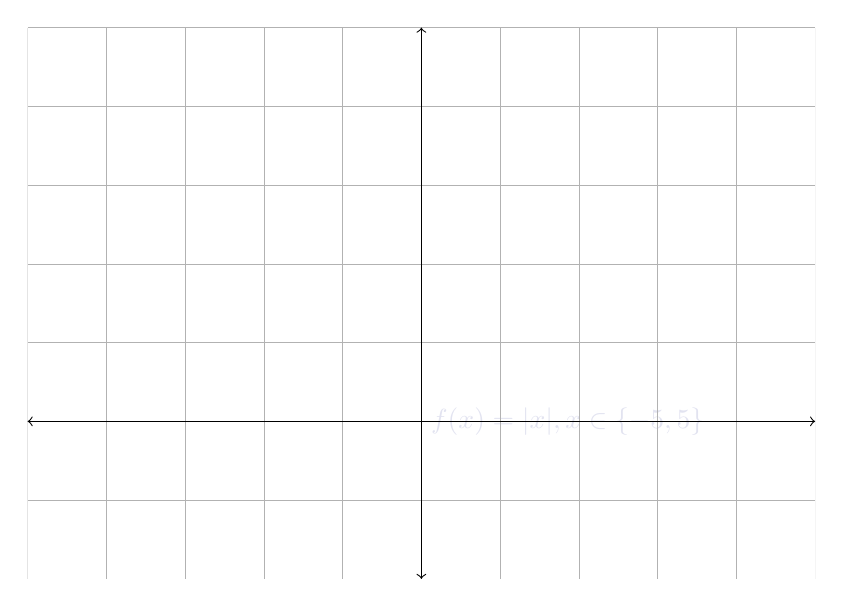
\begin{tikzpicture}[scale=1]
 \def\xmin{-5}
 \def\xmax{5}
 \def\ymin{-2}
 \def\ymax{5}
 \clip
   (\xmin,\ymin) rectangle (\xmax,\ymax);
 \filldraw[fill=blue,fill opacity=0.15, color=neekiBlue, <->, variable=x]
   plot[id=parabola, raw gnuplot, smooth]
   function{
     set xrange [\xmin:\xmax];
     set yrange [\ymin:\ymax];
     plot abs(x);}
   node[right] {$f(x) = |x|, x \in \{ -5,5 \} $};
 % grid
 \draw[very thin, color=black!30, ystep=1, xstep=1]
   (\xmin,\ymin) grid (\xmax,\ymax);
 % x-axis
 \draw[<->]
   (\xmin,0) -- (\xmax,0) node[right] {$x$};
 % y-axis
 \draw[<->]
   (0,\ymin) -- (0,\ymax) node[above] {$f(x)$};
\end{tikzpicture}
\caption{A function of absolute value: $f(x) = |x|$}
\end{figure}
An absolute function in the form $ f(x) = |x|$
\begin{table}[!hbt]
\label{tab:PartsOfAnAbsoluteFunction}
\begin{tabularx}{\linewidth}{| l X |}
  \hline
  \multicolumn{2}{|l|}{Where:} \\
  \hline \hline
  m & represents a component of the gradient (covered more in Chapter
  \ref{chap:Differentiation} ``Differentiation''). \\
  x & is the independent variable \\
  y & is the dependent variable \\
  x & is the independent variable \\
  y & is the dependent variable \\
\hline
\end{tabularx}
\end{table}
\clearpage
%-----------------------------------------------------------------------------%
%- Calculus :: Lines & Limits ------------------------------------------------%
%-----------------------------------------------------------------------------%
\newpage
\section{Limits}
\label{sec:Limits}
There are some types of functions you may be asked to evaluate for various
values of $x$ which are unreasonable. One such example is the hyperbolic
function $f(x) = \frac{1}{x} $ where $x = 0$. In MATH130, we consider this value
an illegal or ``undefined'' value - but there is still a way to evaluate it.
Consider taking a table of values\ref{tab:LimitsHyperbolaExample}:
\begin{table}[!hbt]
\label{tab:LimitsHyperbolaExample}
\begin{tabularx}{\textwidth}{| c || r | r | r | r | r | r | r | r | r | r | X |}
  \hline
  x & 5    & 4    & 3    & 2    & 1    & 0.8  & 0.6  & 0.4  & 0.2  & 0.1 & \ldots \\
  \hline
  y & 0.20 & 0.25 & 0.33 & 0.50 & 1.00 & 1.25 & 1.67 & 2.50 & 5.00 & 10.00 &
  \ldots \\
  \hline
\hline
\end{tabularx}
\caption{Table of values for hyperbolic function $f(x) = \frac{1}{x}$}
\end{table}
Note how as $x$ gets smaller, $y$ gets bigger. The way this is formally worded
is ``as $x$ approaches $0$, $y$ approaches infinity, and written:
\begin{align}
  x \to 0 & \; f(x) \to \infty
\end{align}
From this point, we can see that $x$ cannot be zero, however all other
$\mathbb{R}$ are acceptable. Building on this we can define it as a set:
\begin{align}
  & x \to 0 \; f(x) \to \infty \nonumber \\
  & x \in \{ \mathbb{R}, x \neq 0 \}
\end{align}
The key to understanding how limits work is to identify what $x$ values are
undefined or otherwise illegal. Key indicators of this phenomena are when you
see $x$ inside a squareroot sign, or as a divisor in a quotient: 

%-----------------------------------------------------------------------------%
%- Calculus :: Differentiation -----------------------------------------------%
%-----------------------------------------------------------------------------%
\newpage
\chapter{Differentiation}
\label{sec:Differentiation}
In overly simplified terms, differentiation is the process of taking a curve
on a graph and finding what the gradient of that curve is. There are 4
methods which are useful for MATH130. These are:
\begin{itemize}
  \item Power Method (well, that's what I call it)
  \item Product Rule
  \item Quotient Rule
  \item Chain Rule
\end{itemize}
Because the notion of calculus was a joint effort between several
mathematicians\footnote{Gottfried Leibniz woke up one day and thought ``I'm
going to invent a whole new branch of mathematics to annoy students for the
next few hundred years.'' Approximately 10 years earlier, Sir Isaac Newton
thought ``I know what will really get Leibniz's goat... I'll get the drop on
him with this idea I have.'' Consequently, the two never became friends.}
operating in secret, and without a project manager there are two important
notations.\footnote{there are more, but we don't need to know about them for
MATH130}
\\
The first notation is the ``dash'', ``prime'', or ``Lagrange's'' notation and
appears as such:
\begin{align}
   f(x) & = ... \\
  f'(x) & = ...
  \intertext{Secondly is Leibniz's notation:}
  \derivative f(x) &= ...
  \intertext{Euler's notation: (not so common in MATH130)}
   Df(x) & = ... \\
\end{align}
Each notation has their merits and usefulness; Lagrange's form is neat and
compact for simple derivatives, however Leibniz's notation describe what is
being differentiated and what is in respect to, which is useful for the chain
rule discussed shortly. As such, it is important to be familiar with all the
above forms as they will often be used interchangeably for brevity,
neatness and ease of memorising them. In terms of how you answer a question - 
if there is no stated style of notation, go for what ``looks'' like it works
\footnote{Munner's Law: If it looks wrong it probably is. -- Cliff Munro,
1996 Cranbrook School, Design and Technology teacher. Author's corollary: If it
doesn't look wrong, hopefully it's right.} and is clear and neat. Clear and
neat usually results in the marker understanding what you are on about, so even
if you are wrong, you might get partial marks.
\\
A useful tip, when you are first getting used to differentiation, it may be
handy to use Leibniz's notation and say in your mind what you are
differentiating, and what it is in respect to.
%-----------------------------------------------------------------------------%
%- Calculus :: Differentiation :: Power Method -------------------------------%
%-----------------------------------------------------------------------------%
\section{Power Method}
\label{sec:PowerMethod}
The power method is by far the easiest to understand of all 3 methods, and if
possible, it may be easier to rearrange a part of an equation into index
notation and differentiate that way. This method is not always possible,
but by using the power laws from the series of equations starting with
\ref{eq:IndexLaw_Power0}, sometimes a shortcut can be made, which is why
Section \ref{sec:ExponentialsAndLogarithms} important to know very well.
\\
Put simply, the power method can be understood as ``multiply the base by the
power and subtract one from the power'', and is demonstrated in equation
\ref{eq:DiffPowerMethod} below.
\begin{align}
  f(x) & =   {x}^{a} + k \label{eq:DiffPowerMethodKValue} \\
  \derivative f(x) & =   a{x}^{a-1} \label{eq:DiffPowerMethod}
\end{align}
The value $k$ represents a constant, often just a plain number, though it
doesn't have to be. The important thing about the $k$-value in this example is
that there is no $x$ component. Hence it ``disappears''.\\
Functions may have more than one term, consider the following quadratic:
\begin{align}
  f(x)             & = {x}^{2} + 2xb + {b}^{2} \\
  \derivative f(x) & = 2{x}^{1} + 2b \\
                   & = 2(x+b) \label{eq:DiffPowerMethodRespectTo}
\end{align}
Here we are asked to differentiate with respect to $x$ (denoted by the symbol
$\derivative$). To do this, we bring the power of ${x}^{2}$ to the front, and
subtract 1 to give $2{x}^{1}$, and we do the same for the term ${2xb}$ by
looking at the invisible power (it's there, we just don't write it out of
laziness!\footnote{Or convenience, neatness, brevity.}): $2*{x}^{1}*b$
%-----------------------------------------------------------------------------%
%- Calculus :: Differentiation :: Product Rules ------------------------------%
%-----------------------------------------------------------------------------%
\section{Product Rule}
\label{sec:ProductRule}
A function $f(x)$ is a product of two functions, $u(x) * v(x)$. For example:
\begin{align}
  f(x) & = {x}^{3} \sin(x) \label{eq:DiffProdEx1}\\
       & = u(x)v(x)
\end{align}
In this case, we can see that $u(x) = {x}^{3}$ and $v(x) = \sin(x)$. While there
is a mathematical proof\footnote{refer to section \ref{eq:ProofOfProductRule} of
appendix} it is not necessary for MATH130. All we need to know is:
\begin{align}
              f(x) & = u(x)*v(x) \\
  \derivative f(x) & = u'(x)*v(x) + v'(x)*u(x)
\end{align}
So for \ref{eq:DiffProdEx1}, to find the derivative:
\begin{align}
              f(x) & = {x}^{3}\,\sin(x) \nonumber \\
  \derivative f(x) & = \derivative ({x}^{3}) * \sin(x) +
                       {x}^{3} * \derivative (\sin(x)) \\
                   & = {3x}^{2}*\sin(x) + {x}^{3}*\cos(x)
\end{align}
This example makes use of a derivative of a trigonometric function. This will be
explored in chapter \ref{chap:DifferentiationOfTrigFunctions}, ``Differentiation
of Trig Functions'' - until then, just ignore the trigonometric part.
%-----------------------------------------------------------------------------%
%- Calculus :: Differentiation :: Quotient Rule ------------------------------%
%-----------------------------------------------------------------------------%
\section{Quotient Rule}
\label{sec:QuotientRule}
A quotient is a division - just like from primary school: $\frac{u}{v}$.
Previously we may have called the $u$ part the numerator, nowadays it is
called the \emph{dividend}, and the $v$ denominator previously called the
denominator is now called the \emph{divisor}, with the \emph{quotient} being
the result.
\\
To do quotient rule differentiation, we are actually using a modified version
of the product rule, however for MATH130 it is only required to think of it as a
separate rule.\footnote{Mathematical proof of this is in section 
\ref{eq:ProofOfQuotientRule} of the appendix.} The rule takes the form of:
\begin{align}
  f(x) & = \frac{u}{v} \\
  f(x)\derivative & = \frac{u\derivative\,v - u\,v\derivative}{{v}^{2}}
                      \label{eq:DiffQuot1}
  \intertext{ Although both \ref{eq:DiffQuot1} and \ref{eq:DiffQuot2} are
  identical, \ref{eq:DiffQuot2} is tidier, and may be easier to remember.}
  f'(x) & = \frac{u'\,v - u\,v'}{{v}^{2}} \label{eq:DiffQuot2}
\end{align}
Consider the following example:
\begin{align}
  f(x)  & = \frac{{x}^{2}}{4x} \\
  f'(x) & = (4x){x}^{2}\derivative - {x}^{2} (4x\derivative) \\
  f'(x) & = (4x)2x - {x}^{2}\,(4) \\
  f'(x) & = 8{x}^{2} - 4{x}^{2} \\
  f'(x) & = 4{x}^{2}
\end{align}
%-----------------------------------------------------------------------------%
%- Calculus :: Differentiation :: Chain Rule ---------------------------------%
%-----------------------------------------------------------------------------%
\newpage
\section{Chain Rule}
\label{sec:ChainRule}
The chain rule is useful for differentiation a function $f(x)$ where there are
functions inside of functions (such as $\ln(\sin(x))$). To do this, we break
the function up into it's components, give them some names \footnote{''
\emph{Let}`` is possibly the most important word you will come across in
mathematics. You can use it to redefine stuff if it's too complex and break it
into smaller manageable pieces and put it back together again." -- Chris
Gordon, MATH130 lecturer, Macquarie University, 2011} and apply the chain rule.
The rule takes the form as follows:
\begin{align}
  f(x) & = v(u(x)) \\
  f(x)\derivative & = f\derivative[u]\,u\derivative[x] \label{eq:DiffChainRule}
\end{align}
Here is an example of where we might use the chain rule:\footnote{Note that the
$v$ function above in this example is simply ${u}^{3}$.}\footnote{While we
could use the power method to solve this particular problem in 2 steps, we will
demonstrate chain rule first, and then the power method.}
\begin{align}
  f(x) & = {({x}^{2})}^{3}
  \intertext{Let $u = {x}^{2}$ such that}
  f(x) & = {u}^{3} \label{eq:DiffChainRuleLet}
  \intertext{The first step in \ref{eq:DiffChainRuleLet} is to identify the
  chain rule, and to name the function inside $u$. It just makes things
  easier this way for most of the time.}
  f(x)\derivative & = f\derivative[u] * u\derivative[x] \\
                  & = \left[ 3{u}^{2} \right]\,\left[ 2x \right]
  \intertext{\ref{eq:DiffChainRuleLet} It often helps to rewrite the equation
  in terms of $f(x)$ and $u$, and then to write out the chain rule. Normally we
  are differentiating $f(x)$ with respect to $x$ ($\derivative$). Here we
  differentiate $f(x)$ with respect to $u$ (ie $\derivative[u]$) \emph{THEN}
  multiply by $u$. The rest is plain old algebra. So.. substitue values back
  for $u$.}
                  & = \left[ 3{({x}^{2})}^{2} \right] * 2x
  \intertext{simplify the first set of brackets with basic power laws}
                  & = (3{x}^{4})(2x) \\
                  & = 6{x}^{5}
\end{align}
As a point of exercise, here's how much faster it is using the power method:
\begin{align}
  f(x) & = {({x}^{2})}^{3} \\
  f(x)  & = {x}^{6}
  \intertext{Now we use the differentiation power method, bring the power out
  the front and reduce the power by one}
  f(x)\derivative & = 6{x}^{5}
  \intertext{Look! Only two steps!}
\end{align}
It should be noted however, that power method cannot be used for all chain rule
problems (in fact, most of the time it can't - but for easy ones like this, it
is far more efficient to use power method). The following example cannot use
power method, and we \emph{should} use the chain rule:
\begin{align}
  f(x) & = \ln(\sin(x)) \\
  \intertext{Let } u(x) & = \sin(x)
\end{align}
%-----------------------------------------------------------------------------%
%- Calculus :: Differentiation of Exponents and Logs -------------------------%
%-----------------------------------------------------------------------------%
\chapter{TODO: Differentiation of Exponents and Logs}
\label{chap:DifferentiationOfExponentsAndLogs}
%-----------------------------------------------------------------------------%
%- Calculus :: Differentiation of Trigonometric Functions --------------------%
%-----------------------------------------------------------------------------%
\chapter{Differentiation of Trigonometric Functions}
\label{chap:DifferentiationOfTrigFunctions}
Consider the plot of the function $f(x) = sinx$
\begin{figure}[!htb]
\label{fig:GraphTemplate}
\begin{tikzpicture}[samples=50,scale=1]
   \draw[color=neekiRed,domain=0:pi,variable=x]
     plot[id=sinx] function{1/x}
     node[right] {$f(x) = \frac{1}{x}, x \in \{ -5,-\frac{1}{5} \} $};
%   \draw[color=neekiBlue,domain=0:5,variable=x]
  \draw[<->]  (0.0,-5.0) -- (0.0,5.0) node[above] {$f(x)$};
  \draw[<->] (-5.0, 0.0) -- (5.0,0.0) node[right] {$x$};
\end{tikzpicture}
\caption{A hyperbolic function: $f(x) = \frac{1}{x}$}
\end{figure}
A hyperbolic function in the form $ f(x) = \frac{1}{x}$
\begin{table}[!hbt]
\label{tab:GraphTemplateParts}
\begin{tabularx}{\linewidth}{| l X |}
  \hline
  \multicolumn{2}{|l|}{Where:} \\
  \hline \hline
  x & is the independent variable\\
  y & is the dependent variable\\
\hline
\end{tabularx}
\end{table}
%
Here are some equations that are handy to remember. Source \cite{RHBDiffQuickStart}.
\begin{align}
  \derivative {x}^{n} & = n{x}^{n-1} \\
  \derivative {\emph{e}}^{ax} & = a{\emph{e}}^{ax} \\
  \derivative ln(ax) & = \frac{1}{x} \\
  \derivative sin(ax) & = (a)cos(ax) \\
  \derivative cos(ax) & = (-a)sin(ax) \\
  \derivative tan(ax) & = (a){sec}^{2}(ax) \\
  \derivative sec(ax) & = (a)sec(ax)tan(ax) \\
  \derivative csc(ax) & = (-a)csc(ax)cot(ax) \\
  \derivative cot(ax) & = (-a){csc}^{2}(ax) \\
  \derivative {sin}^{-1}(\frac{x}{a}) & = \frac{1}{\sqrt[2]{{a}^{2} - {x}^{2}}}
  \\
  \derivative {sin}^{-1}(\frac{x}{a}) & = \frac{-1}{\sqrt[2]{{a}^{2} - {x}^{2}}}
  \\
  \derivative {sin}^{-1}(\frac{x}{a}) & = \frac{a}{\sqrt[2]{{a}^{2} - {x}^{2}}}  
\end{align}
For a proof, refer to appendix section \ref{sec:DiffTrigProof},
``Differentiation of Trig Functions Proof''
%-----------------------------------------------------------------------------%
%- Calculus :: Differentiation Maxima and Minima -----------------------------%
%-----------------------------------------------------------------------------%
\chapter{TODO: Maxima and Minima}
\label{chap:MaximaAndMinima}
%-----------------------------------------------------------------------------%
%- Calculus :: Differentiation of Trigonometric Functions --------------------%
%-----------------------------------------------------------------------------%
\chapter{TODO: Grokking Word Problems}
\label{chap:GrokkingWordProblems}
%-----------------------------------------------------------------------------%
%- Calculus :: Differentiation of Trigonometric Functions --------------------%
%-----------------------------------------------------------------------------%
\chapter{TODO: Newton's Method}
\label{chap:NewtonsMethod}
\begin{align}
  x_1 = x_0 - \frac{f(x_0)}{f'(x_0)}
\end{align}
Newton's Method is used to find successively better approximations of the roots
of a function.

We take a value of $x$, $x_0$ and subtract the function at $x_0$ divided by the
derivative of that function at $x_0$. The result, $x_1$ is an answer close to
the roots of that function.

What we can do next, is put $x_1$ back into the same process and get a better
approximation of the function. If we repeat this over and over, we will either
get an exact value of the roots of the function, or we will get pretty darn
close to it.

%-----------------------------------------------------------------------------%
%- Calculus :: Practical Uses of Differentiation -----------------------------%
%-----------------------------------------------------------------------------%
\chapter{TODO: Practical uses of Differentiation}
\label{sec:PracticalUsesOfDifferentiation}
%-----------------------------------------------------------------------------%
%- Calculus :: Differentiation of Trigonometric Functions --------------------%
%-----------------------------------------------------------------------------%
\chapter{TODO: Integration}
\label{sec:Integration}
tl;dr \emph{Integration is the reverse process of Differentiation.}

Integration is as looking at the \emph{accumulated change}, often by summing (or
subtracting) of a quantity with respect to another quantity.

If we were to delve more into what integration is, then we could describe it as
finding the area ``underneath a curve'' (more precisely, between the curve and
the x-axis).

There are many different ways of doing this, and MATH130 requires we know 2 of
them:
\begin{description}
  \item[Riemann Sums]
  \item[Simpson's Rule]
  \item[Trapezoidal Rule]
\end{description}

There are two types of integration:
\begin{description}
  \item[Anti-derivatives] or \emph{indefinite integrals}
  \item[Definite Integrals]
\end{description}
The principles behind indefinite and definite integrals are the same, however,
with definite integrals, you have a range for which you are integrating your
function, where as indefinite integrals have no range (beyond the complete range
of the function itself).

\section{Riemann Sums}
\begin{enumerate}
  \item Draw a bunch of rectangles from the $x$-axis to the function
such that the top left corner touches the function. This left hand corner is called a
\emph{Left-hand Riemann sum.}

  \item Now draw the same, but with the right hand corner, a ``Right-hand
 Riemann sum''.
\end{enumerate}

For the function $2^x$ divided into 4 rectangles, the area can be calculated as

$L_4 = \frac{1}{2} \left(2^1 + 2^{1.5} + 2^{2} + 2^{2.5}\right) \approx 7.24$
and
$R_4 = \frac{1}{2} \left(2^{1.5} + 2^{2} + 2^{2.5} + 2^{3}\right) \approx 10.24$

\noindent Our intuition tells us to take the mean of these two numbers, however
the curve is not quite straight, so the mean would be slightly larger. This mean
($8.74$). It is pretty close though, and the most you can be wrong by is the
interval of the gap divide by two\ldots That is, $\frac{R_4-L_4}{2} =
\frac{3}{2} = 1.5$.

\noindent Suppose we were to draw more intervals, $L_5$ and $R_5$ would be
closer. $L_{500}$ and $R_{500}$ would be closer again. The error converges to
zero with more rectangles.

\noindent More generally,
\begin{align}
  L_n &= 2^{1\cdot \Delta x} +2^{2\cdot \Delta x} +2^{3\cdot \Delta x} +
  \ldots + 2^{(n-1)\cdot \Delta x} \\
  L_n &= f(1)\Delta x + f(1+\Delta x)\Delta x + \ldots + f(1+(n-1)\Delta
  x)\Delta x \\
  L_n &= \sum_{i=0}^{n-1} f(1 +i\Delta x)\Delta x
\intertext{The exact answer can be given by:}
  A &= \lim_{n \to \infty} \sum_{i=0}^{n-1} f(1+i \Delta x) \Delta x \\
    &= \int_{1}^{3} f(x) dx
\end{align}

\noindent This formula is called ``the definite integral of f from $x=1$ to
$x=3$''.
Where:
\begin{table}[!hbt]
\label{tab:PartsOfAnIntegral}
\begin{tabularx}{\linewidth}{| l X |}
\hline
\multicolumn{2}{|l|}{The convention I will use here is:} \\
\hline \hline
$\int$ & is the integral representing the \emph{sum} \\
$\int_a$ & $a$ is our starting point \\
$\int_{}^b$ & $b$ is our finishing point \\
$f(x)$ & is the function to be integrated \\
$dx$   & is what we are integrating with respect to \\
\hline
\end{tabularx}
\caption{Parts of integrating a function}
\end{table}

\section{General form of a Riemann Sum}
\begin{align}
  L_n &= f(a)\Delta x + f(a + 1 \Delta x)\Delta x + f(a + 2 \Delta x)\Delta x +
  \ldots + f(a + (n-1)\Delta x)\Delta x \\
      &= \sum_{i=0}^{n-1} f(a+i \Delta x)\Delta x \\
      &= \sum \ldots \\
  L_n & \to A ~\text{as} ~ n \to \infty \\
  A &= \lim_{n \to \infty} f(a+i \Delta x)\Delta x \\
    &= \int_a^b f(x) dx
\end{align}

\section{Technique of Integration: Undoing the Chain Rule}
Recall the chain rule:
\begin{align}
  (f \circ g)'(x) &= f'(g(x)) \cdot g'(x) \nonumber \\
\intertext{By reversing we have}
  \int f'(g(x))\cdot g'(x) \nd{x} &= (f \circ g)(x) \\
\intertext{Let}
  f'(g(x)) &= f'(u) \\
  g'(x)\nd{x} &= \nd{u} \\
\intertext{Such that}
\int f'(g(x))\cdot g'(x) \nd{x} &= \\
  &= \int f'(u)\nd{p} \\
  &= f(g(x))
\intertext{This works because $p$ is an inside function, and we can
differentiate it:}
  \deriv{p}{x} &= g'(x) \\
  \nd{p} &= g'(x)\nd{x}
\end{align}

\subsection{Example}
\begin{align}
  \int \left(15x^2 + 4\right)\left(15x^3+4x+1\right)^8\nd{x} &=
  \intertext{Let the inside function, u}
  u &= 5x^3+4x+1 \\
  \intertext{such that}
  \deriv{u}{x} &= 15x^2 + 4 \\
  \nd{u} &= \left(15x^2 + 4\right)\nd{x}
  \intertext{and}
  \int \left(15x^2 + 4\right)\left(15x^3+4x+1\right)^8\nd{x} &= \\
    &= \int u^8\nd{u} \\
    &= \frac{u^9}{9} \\
  \intertext{then substitute back}
    &= \frac{\left(5x^3+4x+1\right)^9}{9}
\end{align}

\subsection{Example}
\begin{align}
  \int \frac{1}{8x-3}\nd{x} &= \int \left(8x-3\right)^{-1}
  \intertext{It is handy to remember:}
    \int \frac{1}{x} \nd{x} &= \log(|x|) \\
  \intertext{let u}
  u &= 8x -3 \\
  \deriv{u}{x} & = 8 \\
  \intertext{thing}
  &= \frac{1}{8} \int \frac{1}{u} \nd{u} \\
  &= \frac{1}{8} \log(|u|) \\
  &= \frac{1}{8} \log(|8x-3|)
\end{align}

Rule to memerise:
\begin{align}
  \int f'(x) e^{f(x)} \nd{x} &= e^{f(x)}
  \intertext{we can get to this via $u$ substition, let}
  u &= f(x) \\
  \deriv{u}{x} &= f'(x) \\ 
  \nd{u} &= f'(x)\nd{x} \\
  \int e^u \nd{x}
\end{align}

\begin{align}
  \int \frac{f'(x)}{f(x)} \nd{x} &= \log(|f(x)|) \\
  \intertext{By:}
   \int \frac{u'}{u} \nd{u} \\
  &= \int \frac{1}{u} \nd{u}
  \intertext{Where}
  u &= f(x)
\end{align}
%-----------------------------------------------------------------------------%
%- Calculus :: Differentiation of Trigonometric Functions --------------------%
%-----------------------------------------------------------------------------%
\chapter{TODO: Trapezoidal Rule}
\label{chap:TrapezoidalRule}
%-----------------------------------------------------------------------------%
%- Calculus :: Differentiation of Trigonometric Functions --------------------%
%-----------------------------------------------------------------------------%
\newpage
\section{TODO: Simpson's Rule}
\label{sec:SimpsonsRule}
%-----------------------------------------------------------------------------%
%- Calculus :: Differentiation of Trigonometric Functions --------------------%
%-----------------------------------------------------------------------------%
\chapter{TODO: Average values of a function}
\label{chap:AverageValuesOfAFunction}
%-----------------------------------------------------------------------------%
%- Calculus :: Differentiation of Trigonometric Functions --------------------%
%-----------------------------------------------------------------------------%
\chapter{TODO: Practical Uses of Integration}
\label{chap:PracticalUsesOfIntegration}

%-----------------------------------------------------------------------------%
%- Appendix ------------------------------------------------------------------%
%-----------------------------------------------------------------------------%
%-----------------------------------------------------------------------------%
%- Appendix :: Trig Identity Quickstart --------------------------------------%
%-----------------------------------------------------------------------------%
\chapter{Trig Identities}
\label{chap:TrigIdentities}
Inverse, quotient, angle sum, and the first primitive identity are the trig
identities are required to memorize. Everything else can be derived.\footnote{However, if you can memorize all of these identities, it may
save crucial seconds in test and exam situations.}

\begin{align}
  \cos \theta & = \frac{y}{1} & = x \\
  \sin \theta & = \frac{x}{1} & = y \\
  \tan \theta & = \frac{y}{x} &
\end{align}

\section{Reciprocal Identities}
\label{sec:TrigReciprocalIdentities}
It should be worth noting the temptation to call these identities the ``inverse
identities'', however, this is technically not true. Inverse identities are not
a part of MATH130 in any of the semesters I have done MATH130, however they will be
included for completeness at the end of this chapter in section
\ref{sec:TrigInverseIdentities}. These are the \emph{reciprocal identities}
because we take the \emph{reciprocal} of an identity.
\begin{align}
  \sec \theta & = \frac{1}{\cos \theta} & = \frac{1}{x} \\
  \csc \theta & = \frac{1}{\sin \theta} & = \frac{1}{y} \\
  \cot \theta & = \frac{\cos \theta}{\sin \theta} & = \frac{1}{\tan \theta} = \frac{x}{y} \\
\end{align}

% \begin{align}
%  \rsin \theta & = \frac{1}{\sin \theta} = \csc \theta\\
%  \rcos \theta & = \frac{1}{\cos \theta} = \sec \theta\\
%  \rtan \theta & = \frac{1}{\tan \theta} = \cot \theta
% \end{align}

\section{Quotient Identities}
\label{sec:TrigQuotientIdentities}
\begin{align}
  \tan \theta = \frac{\sin \theta}{\cos \theta} \\
  \cot \theta = \frac{\cos \theta}{\sin \theta}
\end{align}

\section{Primitive Identities}
\label{sec:TrigPrimitiveIdentities}
Only the first primitive identity needs to eb memorized, remaining primitives
can be derived from the first.
\begin{align}
  \sin^2 \theta + \cos^2 \theta & = 1 \label{eq:TrigPrimitive}
\end{align}
\begin{align}
  \intertext{Divide \eqref{eq:TrigPrimitive} by $\sin^2$.}
  \sin^2 \theta + \cos^2 \theta & = 1 \nonumber \\
  \frac{\sin^2 \theta}{\sin^2 \theta} + \frac{\cos^2 \theta}{\sin^2 \theta}
    & = \frac{1}{\sin^2 \theta} \\
  1 + \cot^2 \theta
    & = \csc^2 \theta \label{eq:Trig2}
  \intertext{Divide \eqref{eq:TrigPrimitive} by $\cos^2$}
  \sin^2 \theta + \cos^2 \theta
    & = 1 \nonumber \\
  \frac{\sin^2 \theta}{\cos^2 \theta} + \frac{\cos^2 \theta}{\cos^2 \theta}
    & = \frac{1}{\cos^2 \theta} \\
  \tan^2 \theta + 1
    & = \sec^2 \theta \label{eq:Trig3}
\end{align}

\section{Angle Sum Identities}
\label{sec:TrigAngleSumIdentities}
Angle sum identities need to be memorized.
\begin{align}
  \sin(A \pm B)
    & = \sin{A}\cos{B} \pm \cos{A}\sin{B} \\
  \cos(A \pm B)
    & = \cos{A}\cos{B} \mp \sin{A}\sin{B} \\
  \tan(A \pm B)
    & = \frac{\tan{A}\pm\tan{B}}{1 \mp \tan{A}\tan{B}}
\end{align}
Angle sum identities form the basis for the double angle identities. There
should be no need to memorize the double angle identities as they can be derived
from the angle sum identities as $A = B = 2A$.

\section{Double Angle Identity: sin(2A)}
\label{sec:TrigDoubleAngleSin}
\begin{align}
  \sin(A + A)
    & = \sin(A)\cos(A) + \sin(A)\cos(A) \\
    & = 2\sin(A)\cos(A)
\end{align}

\newpage
\section{Double Angle Identity: cos(2A)}
\label{sec:TrigDoubleAngleCos}
\begin{align}
  \intertext{$\cos(2A)$ has 3 solutions we need to concern ourselves with in
  MATH130. The 2\tsup{nd} and 3\tsup{rd} solutions
  combine rearrangements of the primitive identity \eqref{eq:TrigPrimitive}.}
  \cos(A + A)
    & = \cos(A)\cos(A) - \sin(A)\sin(A) \\
    & = \cos^2(A) - \sin^2(A) \label{eq:TrigDAFirst}
    \intertext{Rearrange \eqref{eq:TrigPrimitive} to make $\sin^2(A)$ the
    subject}
    \sin^2(A) + \cos^2(A) & = 1 \nonumber \\
    \sin^2(A) & = 1 - \cos^2(A) \\
    \text{sub into \eqref{eq:TrigDAFirst}} \nonumber \\
    & = \cos^2(A) - \sin^2(A) \nonumber \\
    & = \cos^2(A) -(1 - \cos^2(A)) \\
    & = 2\cos^2(A) - 1
    \intertext{Rearrange \eqref{eq:TrigPrimitive} to make $\cos^2(A)$ the
    subject}
    \sin^2(A) + \cos^2(A) & = 1 \nonumber \\
    \cos^2(A) & = 1 - \sin^2(A) \\
    \text{sub into \eqref{eq:TrigDAFirst}} \nonumber \\
    & = \cos^2(A) - \sin^2(A) \nonumber \\
    & = (1 - \sin^2(A)) - \sin^2(A) \\
    & = 1 - 2\sin^2(A)
\end{align}

\newpage
\section{Double Angle Identity: tan(2A)}
\label{sec:TrigDoubleAngleTan}
\begin{align}
  \tan(A + A)
    & = \frac{\tan{A} + \tan{A}}{1 - \tan{A}\tan{A}} \\
    & = \frac{2\tan{A}}{1 - \tan^2{A}}
\end{align}

\section{Trigonometric Calculus Identities}
\label{sec:TrigCalculus}
Think of differentiation of trig functions as a loop with 4 steps, and each time
you differentiate, you have a different value which is fed into the next step of
differentiation. When you reach the last point, you are back where you
started.
\begin{align}
  \deriv{\sin{x}}{x}  & = \cos{x} \\
  \deriv{\cos{x}}{x}  & = -\sin{x} \\
  \deriv{(-\sin{x})}{x} & = -\cos{x} \\
  \deriv{(-\cos{x})}{x} & = \sin{x}
\end{align}
There are 4 quadrants to the unit circle, and differentiation is the process
where by we find the gradient of a function at a point $\theta$. Keep referring
back to figure \ref{fig:TrigCalcSinxCosx} for this next part:  
 \begin{figure}[!htb]
  \begin{center}
    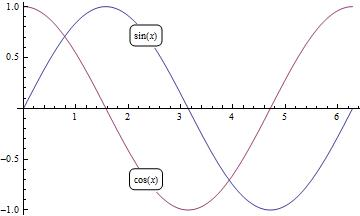
\includegraphics{img/sinxcosx}
    \caption{$\sin(x)$ and $\cos(x)$}
    \label{fig:TrigCalcSinxCosx}
  \end{center}
\end{figure}
\begin{enumerate}
  \item Consider the gradient of $\sin(0)$. $\sin(x)$ is at $(0,0)$ and it has a
  gradient that is at it's steepest: 1. Note how $\cos(0)=1$.
  \item Consider the gradient of $\sin(\frac{\pi}{2})$. $sin(x)$ is at a maximum
  at point $(\frac{\pi}{2},1)$, and the gradient is $0$. Note how
  $\cos(x)$ is plotted and when evaluated $\cos(\frac{\pi}{2})=0$.
  \item Consider the gradient of $\sin(\pi)$. $sin(x)$ is zero, and is at it's
  steepest ``downward slope''. Note how $\cos(x)$ is plotted and evaluated
  $\cos(\pi)=-1$.
  \item Consider the gradient of $\sin(\frac{3\pi}{2})$. $\sin(x)$ is at a
  minimum at point $(\frac{3\pi}{2},-1)$, and $\cos(x)$ is plotted and
  evaluated as $\cos(\frac{3\pi}{2})=0$.
\end{enumerate}
The next step would be to analyse the gradient of $\cos(x)$. One would find that
at any arbitrary point, the gradient of $\cos(x)$ will equal the value of
$\sin(x) \cdot -1$.

\section{Inverse Identities}
\label{sec:TrigInverseIdentities}
An inverse trig function can be though of as an ``undoing function'' for a trig
function.\footnote{This is much like how a logarithm is the undoing function for
an exponent.} All of the inverse trig functions are called
``arc<function>''. The inverse functions hold true iff $-\frac{\pi}{2} \leq
\theta \leq \frac{\pi}{2}$.
\begin{align}
  \sin(\arcsin \theta) &= \theta&\Longrightarrow&&\arcsin(\sin \theta)=\theta \\
  \cos(\arccos \theta) &= \theta&\Longrightarrow&&\arccos(\cos \theta)=\theta \\
  \tan(\arctan \theta) &= \theta&\Longrightarrow&&\arctan(\tan \theta)=\theta \\
  \sec(\arcsec \theta) &= \theta&\Longrightarrow&&\arcsec(\sec \theta)=\theta \\
  \csc(\arccsc \theta) &= \theta&\Longrightarrow&&\arccsc(\csc \theta)=\theta \\
  \cot(\arccot \theta) &= \theta&\Longrightarrow&&\arccot(\cot \theta)=\theta
\end{align}

%-----------------------------------------------------------------------------%
%- Appendix :: Proof of Product Rule -----------------------------------------%
%-----------------------------------------------------------------------------%
\newpage
\subsection{Proof of Product Rule}
\label{sec:ProofOfProductRule}
\begin{align} 
  \label{eq:ProofOfProductRule}
  x & = 1
\end{align}
%-----------------------------------------------------------------------------%
%- Appendix :: Proof of Quotient Rule ----------------------------------------%
%-----------------------------------------------------------------------------%
\newpage
\subsection{Proof of Quotient Rule}
\label{sec:ProofOfQuotientRule}
\begin{align}
  \label{eq:ProofOfQuotientRule}
  x & = 1
\end{align}
%-----------------------------------------------------------------------------%
%- Appendix :: Proof of Chain Rule -------------------------------------------%
%-----------------------------------------------------------------------------%
\newpage
\subsection{Proof of Chain Rule}
\label{sec:ProofOfChainRule}
\begin{align}
  \label{eq:ProofOfChainRule}
  x & = 1
\end{align}
%-----------------------------------------------------------------------------%
%- Appendix :: Differentiation Quickstart ------------------------------------%
%-----------------------------------------------------------------------------%
\newpage
\section{Differentiation of Trig Functions Proof}
\label{sec:DiffTrigProof}
If we have the function $f(x) = sinx$, and take two points, $P$ and $Q$ where
$P = (x,f(x))$ and $Q = (x+h, f(x+h)$ where $h \neq 0$ we can construct a line
joining $P$ and $Q$, and the gradient of this line is given by the ``rise
over run'' formula:
\begin{align}
  \frac{\Delta Y}{\Delta X} & = \frac{f(x+h) - f(x)}{(x+h) - x} \\
                            & = \frac{sin(x+h) - sinx}{h}
\end{align}

%-----------------------------------------------------------------------------%
%- Acknowledgments -----------------------------------------------------------%
%-----------------------------------------------------------------------------%
%-----------------------------------------------------------------------------%
%- Acknowledgments -----------------------------------------------------------%
%-----------------------------------------------------------------------------%
\chapter{Acknowledgements}
\label{chap:Acknowledgements}
I had a whole swag of people to help me along the way. Listed, in no particular
order (because there is no fair way to order you), they are:
\begin{description}
  \item[Carl Svensson] Macquarie University, for the \LaTeX help, the maths, and
  the many late night sessions over a family dinner box, and the many in-jokes
  and innuendoes\footnote{Giggity}.
  
  \item[Michael Griffin, Josh Larietti, Gareth Richardson, Rajika Kuruwita,
  Justin Byrne] Macquarie University, for proof reading, finding errors, and
  being honest\footnote{blunt} when something could be improved\footnote{ie,
  if it was ``shit'', you'd call it ``shit'' ;)}, the many in-jokes, robot
  building, over-eating of junk food, maths, hijinx, sounding out of ideas and
  whatever else goes into peer assisted learning into all hours of the night.
  
  \item[The Heimlich Family] Macquarie University, for giving me a fantastic
  opportunity to put things I've learned into practice, for the life lessons
  that resulted from it. To Mike, Luan, Sarah and Jaye for making FIRST happen
  in Australia, and for inviting me to join the FIRST family.
  
  \item[Dom Verity] Macquarie University, for being a source of inspiration and
  convincing me to try\{\} just one more time before I threw an exception.
  
  \item[MQ Deptartment of Electronics Engineering staff]\footnote{Ana, without
  you, we could never get anything done} David Wong, Yinan, Sam, Tony, Rein,
  Barry, Gengfa, Dush, Hoque, Karu - for making engineering awesome!
  
  \item[MQ Department of Mathematics staff] In particular Fran Grifin, Chris
  Gordon, Rod Yager, Geoff, Dilshara Hill, and Daniel Linssen. You make maths
  comprehensible\footnote{for the most part!}.
  
  \item[FIRST Team 3132] The Thunder Down Under, for always holding me to high
  standards of Gracious Professionalism\texttrademark\footnote{Gracious
  Professionalism is a common law trademark of the United States Foundation for
  Inspiration and Recognition of Science and Technology (US FIRST).}
  
  \item[Mark Leon] NASA, for the words of inspiration and wisdom when you
  spoke at the 2011 Honolulu FIRST FRC regionals:
  ``\ldots at the end of the day, it will be the engineers who save the world
  \ldots This is why we do the math\ldots''
  
  \item[Donald Knuth] for giving me \LaTeX to typeset this book, The Art of
  Computer Programming and Concrete Mathematics as reference materials, as well
  as the awesomeness you've contributed to computing and maths in general.
  
  \item[Celeste Cohen] For letting me show off stuff to you which I thought
  was pretty cool, whilst boring you to tears, as well as advice on the page
  layout and wording. For the Millie. But above all, for being there. /me hugs
  you
  
  \item[Millie] 4 teh nyanz, teh meowz, teh nomz, teh sitz, teh warmz, teh
  purrrrz, and for\footnote{alwayz!} waking me up 45 minutez before teh
  alarm wuz due 2 go off, bcz u wantz 2 play wif u and teh jingly ball.
  
  \item[Pit Crew] it would be remiss of me to not mention the pit crew who make
  sure that I keep going lap after lap\ldots Nathan, Nick, Diana, Heidi, Hugh,
  The Gordon Family\footnote{Put a donk on it!}, Nadia, Martin and Jessica,
  Frankie, the hams at VK2BV, Stephen VK2TQ, Will, Pippa, David, Emily, Andrew,
  John, Sue, Matthew, Richard, my brother Sean, and my mother and my father.
\end{description}
% References
% Bibliography
\bibliography{MATH130}
\bibliographystyle{abbrvnat}
%
\end{document}